\documentclass[11pt,twoside,openright]{book}
% Preamble for "The How To Kernel Borderlands Book" -- Field Manual.
% Built with LuaLaTeX; fonts are the Latin Modern OpenType set shipped with
% TeX Live, so the manual rebuilds anywhere. Pure black and white (grays only).
\usepackage{fontspec}
\setmainfont{lmsans10-regular}[Extension=.otf,UprightFont=lmsans10-bold,
  BoldFont=lmsans10-bold,ItalicFont=lmsans10-boldoblique,BoldItalicFont=lmsans10-boldoblique]
\setsansfont{lmsans10-regular}[Extension=.otf,UprightFont=lmsans10-bold,
  BoldFont=lmsans10-bold,ItalicFont=lmsans10-boldoblique,BoldItalicFont=lmsans10-boldoblique]
\setmonofont{lmmono10-regular}[Extension=.otf,UprightFont=lmmonolt10-bold,
  BoldFont=lmmonolt10-bold,ItalicFont=lmmonolt10-boldoblique,BoldItalicFont=lmmonolt10-boldoblique,Scale=0.98]
\usepackage[a4paper,inner=26mm,outer=20mm,top=26mm,bottom=28mm,headheight=15pt]{geometry}
\usepackage{microtype}
\usepackage{xcolor}
\definecolor{ink}{gray}{0}
\definecolor{ash}{gray}{0.93}
\definecolor{mist}{gray}{0.80}
\definecolor{slate}{gray}{0.35}
\usepackage{graphicx,booktabs,longtable,array,tabularx,enumitem,url,fancyhdr,titlesec,setspace,etoolbox}
\urlstyle{tt}
\newcolumntype{L}[1]{>{\raggedright\arraybackslash}p{#1}}
\newcolumntype{Y}{>{\raggedright\arraybackslash}X}
\setlist{itemsep=2pt,topsep=4pt,parsep=0pt}
\usepackage{listings}
\usepackage[most]{tcolorbox}
\usepackage{tikz}
\usetikzlibrary{positioning,arrows.meta,shapes.geometric,fit,calc,backgrounds,decorations.pathreplacing,matrix,patterns}
\usepackage[pdfusetitle,hidelinks,bookmarksnumbered]{hyperref}
\usepackage{bookmark}
\setstretch{1.08}
\setlength{\parindent}{0pt}
\setlength{\parskip}{6pt}
\emergencystretch=2em
\raggedbottom

% ---- distro switch ---------------------------------------------------------
% latexmk -jobname=... -lualatex="lualatex %O '\def\KBDISTRO{ubuntu}\input{%S}'"
\ifdefined\KBDISTRO\else\def\KBDISTRO{arch}\fi
\def\kbtmp{arch}
\newif\ifarch
\ifx\KBDISTRO\kbtmp\archtrue\else\archfalse\fi
\newcommand{\distroname}{\ifarch Arch Linux\else Ubuntu 24.04 LTS\fi}
\newcommand{\distroshort}{\ifarch Arch\else Ubuntu\fi}
\newcommand{\pkgfile}{\ifarch\path{kernel-borderlands-0.1.0-1-x86_64.pkg.tar.zst}\else\path{kernel-borderlands_0.1.0_amd64.deb}\fi}
\newcommand{\pkgext}{\ifarch\path{.pkg.tar.zst}\else\path{.deb}\fi}

% ---- semantic macros -------------------------------------------------------
\DeclareRobustCommand{\file}[1]{\path{#1}}
\DeclareRobustCommand{\cmd}[1]{\texttt{#1}}
\DeclareRobustCommand{\unit}[1]{\texttt{#1}}
\newcommand{\kb}{Kernel Borderlands}
\newcommand{\todo}[1]{}

% ---- listings --------------------------------------------------------------
\lstdefinestyle{kb}{basicstyle=\ttfamily\footnotesize,columns=fullflexible,keepspaces=true,
  breaklines=true,breakatwhitespace=false,postbreak=\mbox{\textbullet\space},
  frame=single,rulecolor=\color{ink},framesep=5pt,framerule=0.8pt,
  backgroundcolor=\color{ash},xleftmargin=0pt,xrightmargin=0pt,
  showstringspaces=false,upquote=true,aboveskip=8pt,belowskip=8pt,
  literate={—}{{--}}1 {§}{{S.}}1 {→}{{->}}2}
\lstdefinestyle{console}{style=kb,backgroundcolor=\color{white},frame=lines,framerule=1.4pt,
  moredelim=[is][\underbar]{@@}{@@}}
\lstdefinestyle{conf}{style=kb,numbers=left,numberstyle=\tiny\ttfamily,numbersep=6pt,
  stepnumber=5,backgroundcolor=\color{white},frame=single,framerule=1pt,
  morecomment=[l]{\#},commentstyle=\itshape}
\lstset{style=kb}
\newcommand{\lstconf}[3][]{\lstinputlisting[style=conf,caption={#2},label={#3},#1]{../../#2}}

% ---- boxes (black and white) -------------------------------------------------
\newtcolorbox{kbnote}[1][NOTE]{enhanced,breakable,colback=white,colframe=ink,boxrule=0.9pt,
  arc=0pt,left=8pt,right=8pt,top=6pt,bottom=6pt,
  title={#1},fonttitle=\bfseries\sffamily\small,coltitle=white,colbacktitle=ink,
  attach boxed title to top left={yshift=-2.2mm,xshift=4mm},boxed title style={arc=0pt,boxrule=0pt}}
\newtcolorbox{kbwarn}[1][WARNING]{enhanced,breakable,colback=ash,colframe=ink,boxrule=2.2pt,
  arc=0pt,left=10pt,right=8pt,top=8pt,bottom=6pt,
  title={#1},fonttitle=\bfseries\sffamily\small,coltitle=white,colbacktitle=ink,
  attach boxed title to top left={yshift=-2.6mm,xshift=4mm},boxed title style={arc=0pt,boxrule=0pt}}
\newtcolorbox{kbtip}[1][FIELD TIP]{enhanced,breakable,colback=white,colframe=ink,boxrule=0.9pt,
  arc=0pt,left=8pt,right=8pt,top=6pt,bottom=6pt,
  borderline west={4pt}{0pt}{ink},
  title={#1},fonttitle=\bfseries\sffamily\small,coltitle=ink,colbacktitle=mist,
  attach boxed title to top left={yshift=-2.2mm,xshift=4mm},boxed title style={arc=0pt,boxrule=0.9pt}}
\newcounter{kbstep}
\newcommand{\resetsteps}{\setcounter{kbstep}{0}}
\newcommand{\step}[1]{\refstepcounter{kbstep}\par\vspace{4pt}\noindent
  \tikz[baseline=(n.base)]\node[circle,fill=ink,text=white,inner sep=2.2pt,font=\bfseries\sffamily\small](n){\thekbstep};%
  \hspace{6pt}\textbf{#1}\par\vspace{1pt}}

% ---- headings & page style -----------------------------------------------------
\titleformat{\chapter}[display]{\bfseries\sffamily}
  {\vspace*{-6pt}\rule{\textwidth}{3pt}\\[4pt]\Large\MakeUppercase{\chaptertitlename}\ \thechapter}
  {6pt}{\Huge\MakeUppercase}[\vspace{4pt}\rule{\textwidth}{0.8pt}]
\titlespacing*{\chapter}{0pt}{0pt}{22pt}
\titleformat{\section}{\bfseries\sffamily\Large}{\thesection}{10pt}{}[\vspace{-4pt}\rule{\textwidth}{1.2pt}]
\titleformat{\subsection}{\bfseries\sffamily\large}{\thesubsection}{8pt}{}
\titleformat{\subsubsection}{\bfseries\sffamily\normalsize}{\thesubsubsection}{8pt}{}
\titleformat{\part}[display]{\bfseries\sffamily\centering}{\vspace*{3cm}\rule{\textwidth}{4pt}\\[10pt]\Large\MakeUppercase{\partname}\ \thepart}{12pt}{\Huge\MakeUppercase}[\vspace{10pt}\rule{\textwidth}{1pt}]
\pagestyle{fancy}
\fancyhf{}
\fancyhead[LE]{\bfseries\sffamily\small\thepage\quad\leftmark}
\fancyhead[RO]{\bfseries\sffamily\small\rightmark\quad\thepage}
\fancyfoot[C]{\bfseries\sffamily\scriptsize THE HOW TO KERNEL BORDERLANDS BOOK \textbullet\ \MakeUppercase{\distroshort} EDITION}
\renewcommand{\headrulewidth}{1pt}
\renewcommand{\footrulewidth}{0.4pt}
\fancypagestyle{plain}{\fancyhf{}\fancyfoot[C]{\bfseries\sffamily\small\thepage}\renewcommand{\headrulewidth}{0pt}}

% ---- TikZ house style -----------------------------------------------------------
\tikzset{
  >={Stealth[length=2.6mm]},
  box/.style={draw=ink,line width=1pt,fill=white,rectangle,rounded corners=1.5pt,align=center,
    font=\bfseries\sffamily\footnotesize,inner sep=5pt,minimum height=8mm},
  dark/.style={box,fill=ink,text=white},
  soft/.style={box,fill=ash},
  dashedbox/.style={box,dashed,fill=white},
  group/.style={draw=ink,line width=0.8pt,dashed,rounded corners=3pt,inner sep=8pt},
  flow/.style={->,line width=1pt},
  flowd/.style={->,line width=1pt,dashed},
  lbl/.style={font=\bfseries\sffamily\scriptsize,fill=white,inner sep=1.5pt},
}

% ---- checklist marks ---------------------------------------------------------
\newcommand{\chk}{\tikz[baseline=-0.7ex]\draw[line width=1pt] (0,0) rectangle (2.4mm,2.4mm);}
\newcommand{\kbstar}{\tikz[baseline=-0.55ex]\node[star,star points=5,fill=ink,draw=ink,inner sep=1.5pt]{};}

\title{The Kernel Borderlands}
\author{Field Manual To Approach A Kernel Security Software System}
\begin{document}
\frontmatter
\begin{titlepage}
\thispagestyle{empty}
\centering
\vspace*{8mm}
{\rule{\textwidth}{5pt}\par}
\vspace{10mm}
{\bfseries\sffamily\fontsize{44}{48}\selectfont THE HOW TO\\[4mm]KERNEL\\[4mm]BORDERLANDS\\[4mm]BOOK\par}
\vspace{10mm}
{\rule{\textwidth}{1.5pt}\par}
\vspace{8mm}
{\bfseries\sffamily\Large FIELD MANUAL TO APPROACH A\\KERNEL SECURITY SOFTWARE SYSTEM\par}
\vspace{14mm}
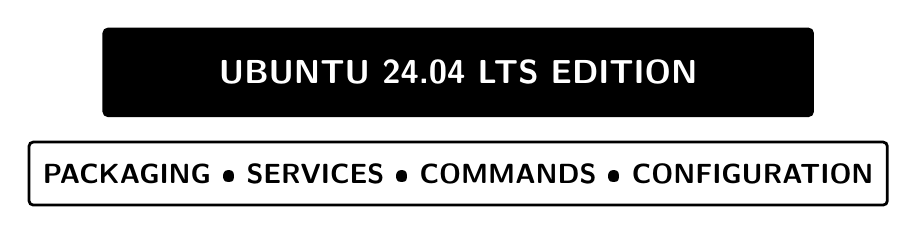
\begin{tikzpicture}
  \node[dark,minimum width=9cm,minimum height=11mm,font=\bfseries\sffamily\large] (a) {\MakeUppercase{\distroname} EDITION};
  \node[box,below=3mm of a,minimum width=9cm,font=\bfseries\sffamily\normalsize] {PACKAGING \textbullet\ SERVICES \textbullet\ COMMANDS \textbullet\ CONFIGURATION};
\end{tikzpicture}
\vfill
{\bfseries\sffamily Package: \pkgfile\par}
{\bfseries\sffamily Release 0.1.0 \textbullet\ Covers kbd, kbd\_sensor, kbctl, kbopd, mcp-server, kb-checker, kb-aads\par}
\vspace{6mm}
{\rule{\textwidth}{5pt}\par}
\end{titlepage}
\mainmatter

\tableofcontents
\part{Orientation}
\chapter{What You Are Operating}
\section{The one-paragraph version}
\kb{} (KB) is a kernel-level runtime defense framework for Linux. A set of \textbf{eBPF sensors} watch kernel
telemetry at Ring~0; a \textbf{Go control plane} (\cmd{kbd}) ingests that telemetry, keeps per-process state,
and enforces policy; a \textbf{Python agent swarm} (\cmd{kb-aads}) coordinates adaptive response; and four
\textbf{operator surfaces} (\cmd{kbctl}, a terminal UI served over SSH, a web dashboard, and an MCP server)
let humans and automation see and steer the system. A separate Rust watchdog (\cmd{kb-checker}) audits the
rest of the stack.

This book is the field manual for \emph{operating the packaged system}: how it is built into a
\pkgext{} package for \distroname, how that package is installed, how every service is started, what every
command does, how the commands combine into working procedures, and what every configuration file means.

\begin{kbwarn}[READ THIS FIRST: THE KB-CHECKER IS DOWN ON PURPOSE]
\cmd{kb-checker}, the safety and integrity watchdog, is \textbf{under maintenance and repairs} and is kept
down in this release. The package installs its binary and unit file, but nothing ever starts it for you:
the package does not enable it (and removes any boot autostart), \cmd{kbctl up} skips it, and \cmd{kbctl status}
prints \texttt{UNDER MAINTENANCE AND REPAIRS (kept down)}. It starts only if you start it by hand. Everything in this book is written for a stack
\emph{without} the watchdog. Chapter~\ref{ch:checker} explains what that means for you.
\end{kbwarn}

\section{The five subsystems}
KB is five subsystems kept in sync through shared wire and event contracts. A change in one often
requires a matching change in another, which is why the package ships them together.

\begin{center}
\small
\begin{tabularx}{\textwidth}{@{}L{3.6cm}L{2.4cm}Y@{}}
\toprule
\textbf{Directory} & \textbf{Language} & \textbf{Role and installed artifact}\\
\midrule
\file{kb-core/} & C (eBPF, CO-RE) & Ring-0 instrumentation and the userspace loader/bridge. Installed as \cmd{kbd\_sensor}.\\
\file{kb-control-plane/} & Go & The \cmd{kbd} daemon: ingestion, storage, scoring, gRPC, HTTP/SSE, enforcement.\\
\file{kb-aads/} & Python & Agent Defense Swarm (multi-agent RL on Ray). Installed as sources plus the \cmd{kbagents} launcher.\\
\file{kb-checker/} & Rust & Stateless safety and integrity watchdog. Installed as \cmd{kb-checker} (\emph{kept down}).\\
\file{kb-op/} & Go / Rust / TS & Operator interfaces: \cmd{kbctl}, \cmd{kbopd} (the TUI and embedded dashboard), \cmd{mcp-server}.\\
\bottomrule
\end{tabularx}
\end{center}

\section{The data flow, end to end}
Figure~\ref{fig:arch} is the picture to keep in your head for the rest of the book. Telemetry flows
\emph{up} from the kernel; containment commands flow \emph{down} on a \emph{separate} socket so a
telemetry burst can never stall or kill delivery of a containment order.

\begin{figure}[ht]
\centering
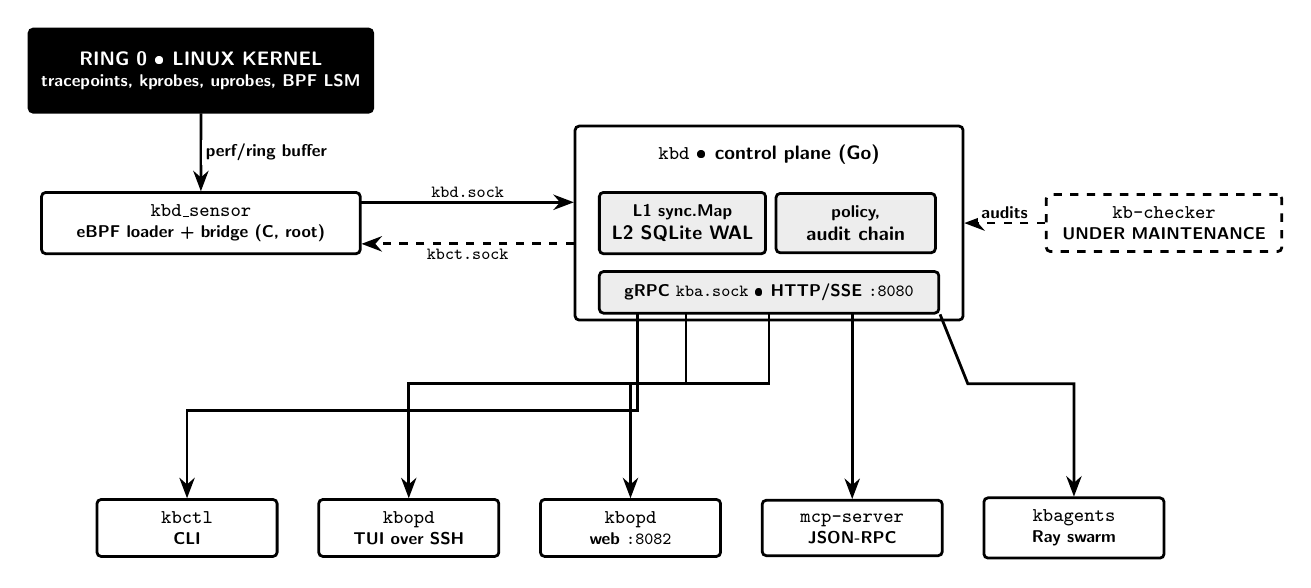
\begin{tikzpicture}[x=1cm,y=1cm,scale=0.88,transform shape]
  % Kernel
  \node[dark,minimum width=4.6cm,minimum height=1.2cm] (kern) at (0,0) {RING 0 \textbullet\ LINUX KERNEL\\[-1pt]\scriptsize tracepoints, kprobes, uprobes, BPF LSM};
  \node[box,minimum width=4.6cm] (sens) at (0,-2.2) {\texttt{kbd\_sensor}\\[-1pt]\scriptsize eBPF loader + bridge (C, root)};
  \node[box,minimum width=5.6cm,minimum height=2.8cm] (kbd) at (8.2,-2.2) {};
  \node[font=\bfseries\sffamily\footnotesize,anchor=north] at (8.2,-0.95) {\texttt{kbd} \textbullet\ control plane (Go)};
  \node[soft,minimum width=2.3cm] (store) at (6.95,-2.2) {\scriptsize L1 sync.Map\\L2 SQLite WAL};
  \node[soft,minimum width=2.3cm] (score) at (9.45,-2.2) {\scriptsize policy,\\audit chain};
  \node[soft,minimum width=4.9cm,minimum height=6mm] (grpc) at (8.2,-3.2) {\scriptsize gRPC \texttt{kba.sock} \textbullet\ HTTP/SSE \texttt{:8080}};
  % operators
  \node[box,minimum width=2.6cm] (ctl) at (-0.2,-6.6) {\texttt{kbctl}\\[-1pt]\scriptsize CLI};
  \node[box,minimum width=2.6cm] (tui) at (3,-6.6) {\texttt{kbopd}\\[-1pt]\scriptsize TUI over SSH};
  \node[box,minimum width=2.6cm] (dash) at (6.2,-6.6) {\texttt{kbopd}\\[-1pt]\scriptsize web \texttt{:8082}};
  \node[box,minimum width=2.6cm] (mcp) at (9.4,-6.6) {\texttt{mcp-server}\\[-1pt]\scriptsize JSON-RPC};
  \node[box,minimum width=2.6cm] (aads) at (12.6,-6.6) {\texttt{kbagents}\\[-1pt]\scriptsize Ray swarm};
  \node[dashedbox,minimum width=3.4cm] (chk) at (13.9,-2.2) {\texttt{kb-checker}\\[-1pt]\scriptsize UNDER MAINTENANCE};
  % flows
  \draw[flow] (kern) -- node[lbl,right]{perf/ring buffer} (sens);
  \draw[flow] ([yshift=3mm]sens.east) -- node[lbl,above]{\texttt{kbd.sock}} ([yshift=3mm]kbd.west);
  \draw[flowd] ([yshift=-3mm]kbd.west) -- node[lbl,below]{\texttt{kbct.sock}} ([yshift=-3mm]sens.east);
  \draw[flow] (grpc.south) ++(-1.9,0) |- (0,-4.9) -| (ctl.north);
  \draw[flow] ([xshift=-1.2cm]grpc.south) -- ++(0,-1) -| (tui.north);
  \draw[flow] ([xshift=0cm]grpc.south) -- ++(0,-1.0) -| (dash.north);
  \draw[flow] ([xshift=1.2cm]grpc.south) -- ++(0,-1.0) -| (mcp.north);
  \draw[flow] (grpc.south east) -- ++(0.4,-1.0) -| (aads.north);
  \draw[flowd] (chk.west) -- node[lbl,above]{audits} (kbd.east);
\end{tikzpicture}
\caption{Data flow. Solid arrows carry telemetry and queries; the dashed arrow from \texttt{kbd} to
\texttt{kbd\_sensor} is the separate control socket that carries containment commands.}
\label{fig:arch}
\end{figure}

\section{The four operator surfaces}
Kernel-level operations demand availability and flexibility, so KB gives you four independent ways in.
If the web port is firewalled you fall back to the SSH TUI; if the shell is restricted, automation
scripts \cmd{kbctl}; if the system is run autonomously, an AI assistant uses the MCP gateway.

\begin{center}
\small
\begin{tabularx}{\textwidth}{@{}L{2.1cm}L{3.2cm}Y@{}}
\toprule
\textbf{Surface} & \textbf{Transport} & \textbf{Use it for}\\
\midrule
\cmd{kbctl} & gRPC over \file{/run/kb/kba.sock} & Scripted playbooks, CI, rapid overrides, starting and stopping the other surfaces.\\
\cmd{kbopd} (TUI) & gRPC over UDS, served via the dedicated operator \cmd{sshd} on port 2222 & Low-bandwidth triage on a bastion, no browser needed.\\
\cmd{kbopd} (web) & Static app on \texttt{127.0.0.1:8082}; REST + SSE to \cmd{kbd} on \texttt{127.0.0.1:8080} & Visual, live threat monitoring.\\
\cmd{mcp-server} & JSON-RPC 2.0 over stdio & AI agents querying state and recommending containment.\\
\bottomrule
\end{tabularx}
\end{center}

\begin{kbnote}[ONE BINARY, TWO FACES]
\cmd{kbopd} is the compiled \cmd{kb-tui} binary installed under another name. Run with a terminal it
draws the TUI; run without one (as the \unit{kbopd.service} unit does) it serves the embedded web
dashboard and starts a background \cmd{mcp-server}. That is why \cmd{kbctl tui} and
\cmd{kbctl dashboard} both end up executing \cmd{kbopd}.
\end{kbnote}

\section{Design invariants you must not break}
\begin{itemize}
\item \textbf{Shared structs stay byte-identical.} Wire structs are packed little-endian on both the C and Go sides (Appendix~\ref{app:wire}). They change together or not at all.
\item \textbf{Rules and policy are compiled, not hand-edited on the sensor.} \file{policy.yaml} and \file{rules.yaml} are read by \cmd{kbd} and \emph{pushed} to the sensor when it connects.
\item \textbf{\cmd{kb-checker} is stateless and has no network listeners.} This is a security invariant of the watchdog, not a style preference.
\item \textbf{Documented contracts beat code.} Where this book and the repository documentation under \file{docs/} disagree, the documentation is canonical and the disagreement is flagged in Chapter~\ref{ch:trouble}.
\end{itemize}

\section{What is verified, and what is not}
A field manual that hides its own uncertainty is dangerous. This release was built and tested without
root access on the build machines, so the status of every claim in this book is one of the following.

\begin{center}
\small
\begin{tabularx}{\textwidth}{@{}L{5.2cm}L{2.4cm}Y@{}}
\toprule
\textbf{Claim} & \textbf{Status} & \textbf{Evidence}\\
\midrule
Both packages build, contain no key material & Verified & File lists inspected; \texttt{find} for \texttt{ssh\_host*}, \texttt{authorized\_keys}, \texttt{id\_*} returns nothing.\\
Ubuntu binaries resolve all libraries on 24.04 & Verified & \texttt{ldd} on every binary, no \texttt{not found}.\\
Unit files rewritten to \file{/usr/bin} & Verified & \texttt{grep ExecStart} on the extracted package.\\
\cmd{kbctl dashboard up/open/down} & Verified & Driven against the packaged \cmd{kbopd} through a stub \cmd{systemctl}; HTTP 200 from the embedded app.\\
SSH TUI path (wrapper, PTY, tabs, quit) & Verified & Unprivileged \cmd{sshd} with the packaged wrapper; exit status 0.\\
Offline banner when \cmd{kbd} is down & Verified & \texttt{[OFFLINE]} and \texttt{[DEMO DATA]} rendered in the TUI.\\
\cmd{kbagents} launcher and \cmd{kb-aads} swarm (Ubuntu) & Verified & Ran on the VM with its venv: status server up, nine agents active, 0 errors, checkpoint loaded. Not run under \cmd{systemd}.\\
\texttt{apt install} / \texttt{pacman -U} on a live host & \textbf{Not tested} & No root in the build session.\\
Units booting under real \cmd{systemd}, eBPF sensor under the package & \textbf{Not tested} & Needs root and a BPF-LSM kernel.\\
\cmd{kbd} HTTP + CORS for the packaged dashboard & \textbf{Source-verified only} & \cmd{kbd} needs a writable \file{/run/kb}.\\
\texttt{operator} account with a \texttt{/bin/sh} shell and \texttt{ForceCommand} (replaces the \texttt{nologin} default) & \textbf{Not tested} & Fix made on the known OpenSSH behaviour; see Chapter~\ref{ch:ssh}.\\
Dashboard action buttons with the runtime token & \textbf{Not tested in a browser} & Build, served bundle, fragment parsing and \cmd{kbctl} hand-off tested; see Chapter~\ref{ch:dash}.\\
\bottomrule
\end{tabularx}
\end{center}
Chapter~\ref{ch:demo} gives you the exact checklist to close every \textbf{Not tested} row on your own host.

\chapter{Ground Truth: Sockets, Ports, Paths, Users}
Everything in later chapters refers back to this chapter. Memorize the shape, look up the details.

\section{Sockets under \file{/run/kb/}}
\file{/run/kb/} is created by \unit{kbd.service} (\texttt{RuntimeDirectory=kb}, mode 0775) and is
removed by systemd when \cmd{kbd} stops.

\begin{center}
\small
\begin{tabularx}{\textwidth}{@{}L{2.3cm}L{3.3cm}L{2.4cm}Y@{}}
\toprule
\textbf{Socket} & \textbf{Direction} & \textbf{Protocol} & \textbf{Purpose}\\
\midrule
\file{kbd.sock} & \texttt{kbd\_sensor} $\to$ \cmd{kbd} & packed structs & Telemetry only, one direction.\\
\file{kbct.sock} & \cmd{kbd} $\to$ \texttt{kbd\_sensor} & packed structs & Containment and sensitive-path pushes. Split from \file{kbd.sock} so a telemetry burst cannot stall containment.\\
\file{kba.sock} & clients $\to$ \cmd{kbd} & gRPC & Enforcement IPC used by \cmd{kbctl}, \cmd{kbopd}, \cmd{mcp-server}, \cmd{kb-aads}.\\
\file{kbc.sock} & \cmd{kb-checker} diagnostics & gRPC & Watchdog diagnostics (unused while the checker is down).\\
\bottomrule
\end{tabularx}
\end{center}

\section{Network ports}
\begin{center}
\small
\begin{tabularx}{\textwidth}{@{}L{1.6cm}L{3.2cm}L{3.5cm}Y@{}}
\toprule
\textbf{Port} & \textbf{Owner} & \textbf{Bind} & \textbf{Notes}\\
\midrule
8080 & \cmd{kbd} HTTP API + SSE & 127.0.0.1 (flag \texttt{--http-addr}) & REST for processes, alerts, logs, services, metrics, agents, policy; SSE on \texttt{/api/events}. CORS allowlist from \texttt{KB\_HTTP\_CORS\_ORIGIN}.\\
8082 & \cmd{kbopd} embedded dashboard & 127.0.0.1, fixed in the binary & Static Vite app plus \texttt{POST /api/containment}.\\
2222 & operator \cmd{sshd} & all interfaces (\texttt{sshd@kb-operator}) & Key-only console that forces the TUI wrapper.\\
8601 & \cmd{kb-aads} status server & 127.0.0.1 (\file{KB_AADS_STATUS_HOST/PORT}) & Agent status; \cmd{kbd} proxies it for \texttt{/api/agents}.\\
\bottomrule
\end{tabularx}
\end{center}
\begin{kbwarn}[PORT 2222 IS THE ONLY NON-LOOPBACK LISTENER]
The dashboard and API bind loopback on purpose. Remote humans reach the system through SSH on 2222
(Chapter~\ref{ch:ssh}) rather than by exposing HTTP. Keep it that way unless you also set
\texttt{KB\_HTTP\_API\_TOKEN} and a TLS-terminating proxy.
\end{kbwarn}

\section{Filesystem layout after install}
\begin{figure}[ht]
\centering
\small
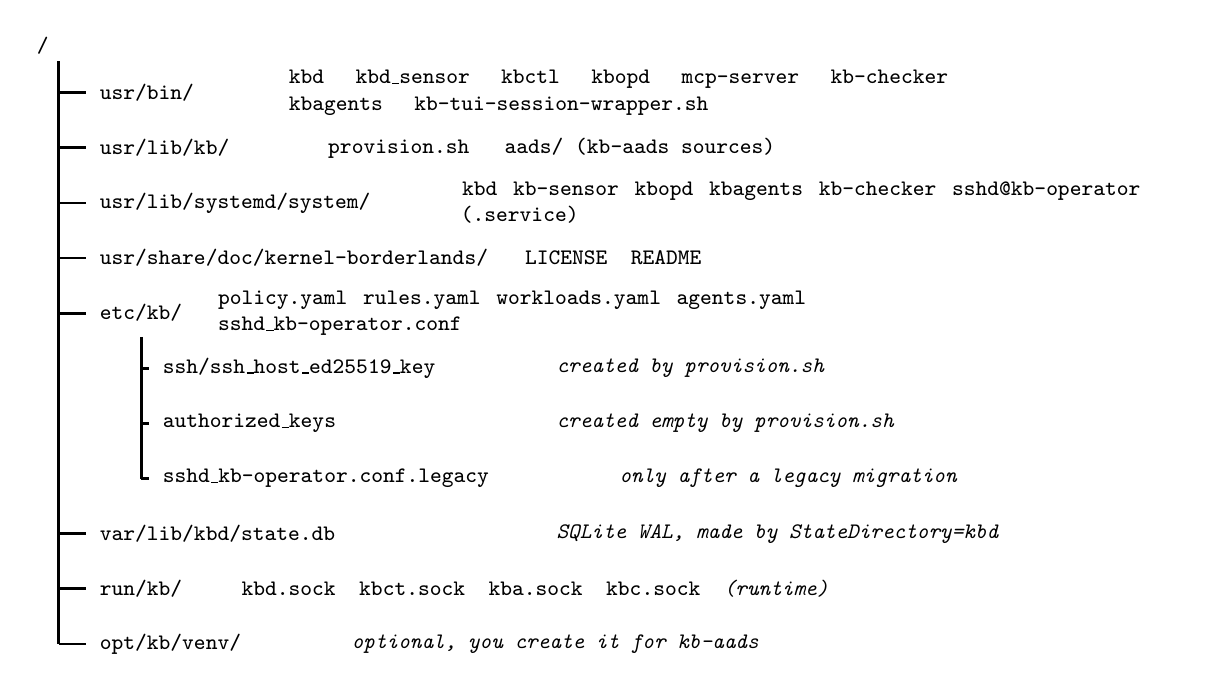
\begin{tikzpicture}[x=1cm,y=1cm]
\tikzset{t/.style={font=\ttfamily\bfseries\footnotesize,anchor=west}}
\node[t] at (0,0) {/};
\node[t] at (0.8,-0.6) {usr/bin/};
\node[t,text width=9cm] at (3.2,-0.6) {kbd \quad kbd\_sensor \quad kbctl \quad kbopd \quad mcp-server \quad kb-checker \quad kbagents \quad kb-tui-session-wrapper.sh};
\node[t] at (0.8,-1.3) {usr/lib/kb/};
\node[t] at (3.7,-1.3) {provision.sh \quad aads/ (kb-aads sources)};
\node[t] at (0.8,-2.0) {usr/lib/systemd/system/};
\node[t,text width=9cm] at (5.4,-2.0) {kbd \ kb-sensor \ kbopd \ kbagents \ kb-checker \ sshd@kb-operator (.service)};
\node[t] at (0.8,-2.7) {usr/share/doc/kernel-borderlands/};
\node[t] at (6.2,-2.7) {LICENSE \ README};
\node[t] at (0.8,-3.4) {etc/kb/};
\node[t,text width=10cm] at (2.3,-3.4) {policy.yaml \ rules.yaml \ workloads.yaml \ agents.yaml \ sshd\_kb-operator.conf};
\node[t] at (1.6,-4.1) {ssh/ssh\_host\_ed25519\_key};
\node[t] at (6.6,-4.1) {\textit{created by provision.sh}};
\node[t] at (1.6,-4.8) {authorized\_keys};
\node[t] at (6.6,-4.8) {\textit{created empty by provision.sh}};
\node[t] at (1.6,-5.5) {sshd\_kb-operator.conf.legacy};
\node[t] at (7.4,-5.5) {\textit{only after a legacy migration}};
\node[t] at (0.8,-6.2) {var/lib/kbd/state.db};
\node[t] at (6.6,-6.2) {\textit{SQLite WAL, made by StateDirectory=kbd}};
\node[t] at (0.8,-6.9) {run/kb/};
\node[t] at (2.6,-6.9) {kbd.sock \ kbct.sock \ kba.sock \ kbc.sock \ \textit{(runtime)}};
\node[t] at (0.8,-7.6) {opt/kb/venv/};
\node[t] at (4.0,-7.6) {\textit{optional, you create it for kb-aads}};
\draw[line width=1pt] (0.4,-0.2) -- (0.4,-7.6);
\foreach \y in {-0.6,-1.3,-2.0,-2.7,-3.4,-6.2,-6.9,-7.6} \draw[line width=1pt] (0.4,\y) -- (0.75,\y);
\draw[line width=1pt] (1.45,-3.7) -- (1.45,-5.5);
\foreach \y in {-4.1,-4.8,-5.5} \draw[line width=1pt] (1.45,\y) -- (1.55,\y);
\end{tikzpicture}
\caption{Where everything lands. Paths are identical on both distributions.}
\end{figure}

\section{Users, groups, and permissions}
\file{provision.sh} runs from the package's post-install step and is idempotent.
\begin{center}
\small
\begin{tabularx}{\textwidth}{@{}L{3.2cm}Y@{}}
\toprule
\textbf{Object} & \textbf{Definition}\\
\midrule
group \texttt{kb} & System group; owns \file{/etc/kb} (mode 0750, \texttt{root:kb}).\\
user \texttt{operator} & System user, no home, member of \texttt{kb}. The only account the operator \cmd{sshd} accepts (\texttt{Match User operator}).\\
\file{/etc/kb/ssh/ssh_host_ed25519_key} & Host key for the operator \cmd{sshd}, generated on first install, never overwritten.\\
\file{/etc/kb/authorized_keys} & Empty at install, \texttt{operator:kb}, mode 0600. Fill it with \cmd{kbctl ssh add-key}.\\
Config files in \file{/etc/kb} & Mode 0640 root-owned; \cmd{kbd} runs as root. Listed as package conffiles so your edits survive upgrades.\\
\bottomrule
\end{tabularx}
\end{center}

\section{Environment variables}
\begin{center}
\small
\begin{tabularx}{\textwidth}{@{}L{4.6cm}L{3.6cm}Y@{}}
\toprule
\textbf{Variable} & \textbf{Read by} & \textbf{Meaning}\\
\midrule
\texttt{KB\_HTTP\_CORS\_ORIGIN} & \cmd{kbd} & Comma-separated browser origins allowed to call the API. The packaged unit sets \texttt{http://127.0.0.1:8082,http://localhost:8082}. Default without it: the Vite dev origins on 5173 only.\\
\texttt{KB\_HTTP\_API\_TOKEN} & \cmd{kbd} & Bearer token gating the mutating routes (\texttt{isolate}, \texttt{restore}). Unset means those routes fail closed.\\
\texttt{KB\_AADS\_STATUS\_HOST}, \texttt{KB\_AADS\_STATUS\_PORT} & \cmd{kbagents} & Bind address of the agent status server (default 127.0.0.1:8601).\\
\texttt{KB\_AADS\_API\_ADDR} & \cmd{kbd} & Where \cmd{kbd} proxies \texttt{/api/agents}; must match the status server.\\
\bottomrule
\end{tabularx}
\end{center}

\chapter{Before You Install: Kernel Prerequisites}\label{ch:prereq}
The package can be installed on any \distroname{} host. The \emph{sensor} will only do its full job on a
kernel that exposes BTF and has the BPF Linux Security Module enabled. Check this first; it takes a minute
and saves an hour.

\section{The checklist}
\resetsteps
\step{Confirm BTF is available}
CO-RE (compile once, run everywhere) relies on kernel type information.
\begin{lstlisting}[style=console]
$ ls -l /sys/kernel/btf/vmlinux
-r--r--r-- 1 root root 5321944 ... /sys/kernel/btf/vmlinux
\end{lstlisting}
If the file is missing, the sensor cannot relocate its programs on this kernel.

\step{Confirm the kernel was built with BPF LSM}
\begin{lstlisting}[style=console]
$ zgrep CONFIG_BPF_LSM /proc/config.gz  # or: grep CONFIG_BPF_LSM /boot/config-$(uname -r)
CONFIG_BPF_LSM=y
\end{lstlisting}

\step{Check whether \texttt{bpf} is in the active LSM list}
\begin{lstlisting}[style=console]
$ cat /sys/kernel/security/lsm
lockdown,capability,landlock,yama,apparmor,bpf
\end{lstlisting}
The trailing \texttt{bpf} means the in-kernel file-access block (\texttt{kb\_lsm\_file\_open}) can attach.
Without it, the sensor still loads its tracing programs; only the LSM program fails to attach, and the
sensor's startup log says so rather than silently doing nothing.

\section{Enabling BPF LSM when it is missing}
Add \texttt{bpf} to the kernel's \texttt{lsm=} boot parameter, regenerate the boot configuration, reboot.

\ifarch
\subsection*{Arch Linux (GRUB)}
\begin{lstlisting}[style=console]
$ sudo $EDITOR /etc/default/grub
  GRUB_CMDLINE_LINUX_DEFAULT="quiet lsm=landlock,lockdown,yama,apparmor,bpf"
$ sudo grub-mkconfig -o /boot/grub/grub.cfg
$ sudo reboot
\end{lstlisting}
\begin{kbnote}[SYSTEMD-BOOT / OTHER LOADERS]
If you use \texttt{systemd-boot}, append the same \texttt{lsm=...} string to the \texttt{options} line of
your entry under \file{/boot/loader/entries/}. Arch's own kernels build BPF LSM in; you only need the
parameter. Keep \texttt{apparmor} in the list only if you actually run it; listing a module your kernel
lacks is harmless but pointless.
\end{kbnote}
\else
\subsection*{Ubuntu 24.04 (GRUB)}
\begin{lstlisting}[style=console]
$ sudo $EDITOR /etc/default/grub
  GRUB_CMDLINE_LINUX_DEFAULT="quiet splash lsm=landlock,lockdown,yama,apparmor,bpf"
$ sudo update-grub
$ sudo reboot
\end{lstlisting}
\begin{kbnote}[UBUNTU 24.04 DEMO VM]
The reference Ubuntu VM runs kernel \texttt{6.8.0-139-generic} and already reports
\texttt{lockdown,capability,landlock,yama,apparmor,bpf} with BTF present, so no change is needed there.
\end{kbnote}
\fi

\step{Verify after reboot}
\begin{lstlisting}[style=console]
$ cat /sys/kernel/security/lsm
\end{lstlisting}
\texttt{bpf} must appear at the end of the list.

\section{What runs where}
\begin{center}
\small
\begin{tabularx}{\textwidth}{@{}L{3.6cm}L{2.6cm}Y@{}}
\toprule
\textbf{Component} & \textbf{Privilege} & \textbf{Why}\\
\midrule
\cmd{kbd\_sensor} & root & Loads eBPF, attaches LSM and uprobes; needs CAP\_BPF, CAP\_PERFMON, CAP\_SYS\_ADMIN (exact set is kernel-dependent).\\
\cmd{kbd} & root & Owns \file{/run/kb}, \file{/var/lib/kbd}, binds the sockets.\\
\cmd{kbopd} (service) & unprivileged-style hardening & Only a loopback listener and a child process.\\
\cmd{sshd@kb-operator} & root, then drops to \texttt{operator} & Standard \cmd{sshd} privilege separation.\\
\bottomrule
\end{tabularx}
\end{center}

\begin{kbwarn}[A VM OR CONTAINER SHARES THE HOST KERNEL ASSUMPTIONS]
Inside a container the sensor sees the \emph{host} kernel. Inside a VM it sees the \emph{guest} kernel, which
is what you want for the demo. Whichever you use, run the checklist above \emph{inside} it.
\end{kbwarn}

\part{Packaging}
\chapter{Anatomy of the Package}
One Makefile target, \cmd{make install-pkg}, defines what ships. Both the \texttt{.deb} and the Arch
package are thin wrappers around it, so the two distributions cannot drift apart.

\section{From source to artifact}
\begin{figure}[ht]
\centering
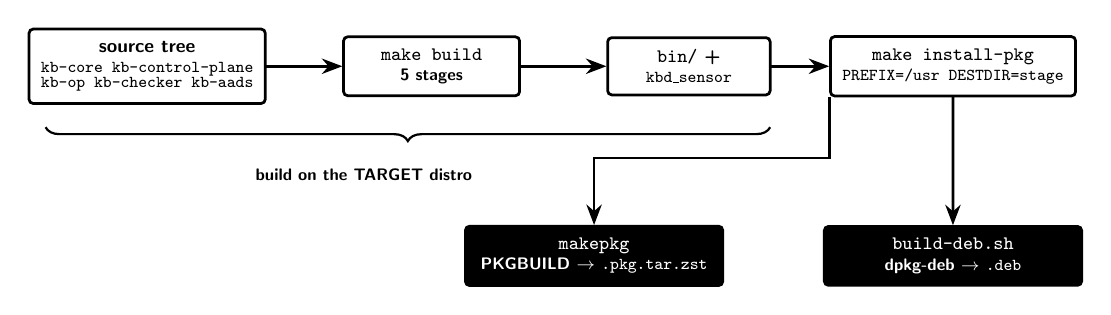
\begin{tikzpicture}[x=1cm,y=1cm,scale=0.86,transform shape]
  \node[box,minimum width=2.6cm] (src) at (0,0) {source tree\\[-1pt]\scriptsize \texttt{kb-core kb-control-plane}\\[-3pt]\scriptsize \texttt{kb-op kb-checker kb-aads}};
  \node[box,minimum width=2.6cm] (build) at (4.2,0) {\texttt{make build}\\[-1pt]\scriptsize 5 stages};
  \node[box,minimum width=2.4cm] (bin) at (8,0) {\texttt{bin/} +\\[-1pt]\scriptsize \texttt{kbd\_sensor}};
  \node[box,minimum width=2.9cm] (stage) at (11.9,0) {\texttt{make install-pkg}\\[-1pt]\scriptsize \texttt{PREFIX=/usr DESTDIR=stage}};
  \node[dark,minimum width=3.8cm] (deb) at (11.9,-2.8) {\texttt{build-deb.sh}\\[-1pt]\scriptsize dpkg-deb $\to$ \texttt{.deb}};
  \node[dark,minimum width=3.8cm] (arch) at (6.6,-2.8) {\texttt{makepkg}\\[-1pt]\scriptsize PKGBUILD $\to$ \texttt{.pkg.tar.zst}};
  \draw[flow] (src) -- (build); \draw[flow] (build) -- (bin); \draw[flow] (bin) -- (stage);
  \draw[flow] (stage) -- (deb);
  \draw[flow] (stage.south west) -- ++(0,-0.9) -| (arch.north);
  \node[lbl] at (3.2,-1.6) {build on the TARGET distro};
  \draw[decorate,decoration={brace,mirror,amplitude=5pt},line width=0.8pt] (-1.5,-0.9) -- (9.2,-0.9);
\end{tikzpicture}
\caption{The packaging pipeline. The brace marks the part that must run on the distribution you are
targeting, because the binaries link the build host's C library.}
\end{figure}

\begin{kbwarn}[BUILD ON THE DISTRIBUTION YOU SHIP TO]
The Go, Rust and C binaries are dynamically linked against the \emph{build host's} glibc. The Arch host that
builds the Arch package has glibc 2.44; Ubuntu 24.04 has 2.39. A binary built on the former will not start
on the latter (``version \texttt{GLIBC\_2.4x} not found''). That is why the \texttt{.deb} is built on the
Ubuntu machine and the Arch package on Arch. Building on the \emph{older} distribution always works
forward; the reverse does not.
\end{kbwarn}

\section{The five build stages}
\cmd{make build} runs these in order and puts every product into the top-level \file{bin/}
(the sensor stays in \file{kb-core/build/}).
\begin{center}\small
\begin{tabularx}{\textwidth}{@{}L{1.2cm}L{3.2cm}Y@{}}
\toprule
\textbf{Stage} & \textbf{Output} & \textbf{What happens}\\
\midrule
1/5 & \file{kb-core/build/kbd_sensor} & \cmd{clang} compiles the BPF programs and userspace loader, \cmd{bpftool} generates the CO-RE skeletons, the vendored \file{libbpf/src/libbpf.a} is linked statically. Hardened with \texttt{-D\_FORTIFY\_SOURCE=3}, stack protector, \texttt{-fPIE}, full RELRO.\\
2/5 & \file{bin/kbd} & \texttt{go build -a} of \file{kb-control-plane/cmd/kbd}.\\
3/5 & \file{bin/kb-checker} & \texttt{cargo build --release} of the watchdog (built even though it is kept down).\\
4/5 & \file{bin/kbctl} & \texttt{go build -a} of the CLI.\\
5/5 & \file{bin/mcp-server}, \file{bin/kbopd} & Builds the MCP server; runs \texttt{npm ci} (only if \file{node_modules} is absent) and \texttt{npm run build} for the dashboard; then \texttt{cargo build --release} of \file{kb-tui}, which \emph{embeds} the dashboard's \file{dist/} at compile time and is copied to \file{bin/kbopd}.\\
\bottomrule
\end{tabularx}
\end{center}
\begin{kbnote}[ORDER MATTERS IN STAGE 5]
The dashboard must be built \emph{before} \cmd{cargo} compiles \file{kb-tui}. The Rust code embeds
\file{kb-dashboard/dist/} with \texttt{rust-embed}; if the folder is missing the compile fails with
``folder ... does not exist''. The Makefile already enforces the order.
\end{kbnote}

\section{The Makefile contract}
\begin{center}\small
\begin{tabularx}{\textwidth}{@{}L{3.3cm}L{3.9cm}Y@{}}
\toprule
\textbf{Variable} & \textbf{Default} & \textbf{Meaning}\\
\midrule
\texttt{PREFIX} & \texttt{/usr/local} & Packages pass \texttt{/usr}.\\
\texttt{BINDIR} & \texttt{\$(PREFIX)/bin} & Where binaries land; also substituted into unit files and the SSH wrapper.\\
\texttt{LIBDIR} & \texttt{\$(PREFIX)/lib} & \file{kb/provision.sh} and \file{kb/aads/}.\\
\texttt{SYSCONFDIR} & \texttt{/etc} & Config root (\file{/etc/kb}).\\
\texttt{UNITDIR} & \texttt{/etc/systemd/system} for \texttt{/usr/local}, else \file{$(PREFIX)/lib/systemd/system} & Where unit files go.\\
\texttt{DESTDIR} & empty & Staging root, prepended to every install path.\\
\texttt{GOARCH} & \texttt{go env GOARCH} & Target architecture of the Go binaries.\\
\bottomrule
\end{tabularx}
\end{center}
\begin{center}\small
\begin{tabularx}{\textwidth}{@{}L{3.3cm}Y@{}}
\toprule
\textbf{Target} & \textbf{Effect}\\
\midrule
\texttt{make build} & The five stages above.\\
\texttt{make install} & Installs the six binaries to \texttt{\$(DESTDIR)\$(BINDIR)}. Historical behaviour: \texttt{sudo make install} still goes to \file{/usr/local/bin}.\\
\texttt{make install-pkg} & \texttt{install} plus the wrapper, \cmd{kbagents}, units (path-rewritten), operator \cmd{sshd} config, default \file{/etc/kb/*.yaml}, \file{provision.sh}, the \cmd{kb-aads} sources, and docs.\\
\texttt{make clean} & Removes build products.\\
\bottomrule
\end{tabularx}
\end{center}

\begin{kbwarn}[THE PACKAGE USES EXPLICIT FILE LISTS ON PURPOSE]
The source tree contains development-only \file{ssh_host_ed25519_key} and \file{authorized_keys} files under
\file{kb-core/} and \file{kb-control-plane/}. They are git-ignored, but they exist on disk. \cmd{install-pkg} names every
file it ships and never copies a directory wholesale (except the \cmd{kb-aads} Python packages, which are
listed folder by folder). If you extend the package, keep it that way and re-run the secrets check in
Section~\ref{sec:secrets}.
\end{kbwarn}

\section{What the unit files are rewritten to}
The sources in \file{packaging/systemd/} use the development path \file{/usr/local/bin}. During
\cmd{install-pkg}, \cmd{sed} rewrites it to \texttt{\$(BINDIR)} (\file{/usr/bin}) in every unit and in the SSH wrapper, and
rewrites the operator \cmd{sshd} config path from \file{/etc/ssh/sshd_config.d/kb-operator.conf} to
\file{/etc/kb/sshd_kb-operator.conf}.

\begin{kbnote}[WHY THE SSHD CONFIG MOVED]
Ubuntu's main \cmd{sshd} reads \texttt{Include /etc/ssh/sshd\_config.d/*.conf}. A file there containing
\texttt{Port 2222} is therefore also loaded by the \emph{host's own} \cmd{sshd}, which grabs port 2222 first;
the dedicated \texttt{sshd@kb-operator} instance then dies with \texttt{Address already in use} and restarts
forever. This was observed on the live Ubuntu VM. The packages avoid it by keeping the file under
\file{/etc/kb/}, where only the dedicated unit reads it.
\end{kbnote}

\section{Package metadata and maintainer scripts}
\begin{center}\small
\begin{tabularx}{\textwidth}{@{}L{3.1cm}L{3.2cm}Y@{}}
\toprule
\textbf{Item} & \textbf{Ubuntu \texttt{.deb}} & \textbf{Arch}\\
\midrule
Source of truth & \file{packaging/deb/} & \file{packaging/arch/PKGBUILD}\\
Runtime deps & \texttt{libc6, systemd, openssh-server, libelf1t64, zlib1g} & \texttt{glibc systemd openssh libelf zlib}\\
Optional & \texttt{python3, python3-venv} (Recommends) & \texttt{python} (optdepends)\\
Config preserved on upgrade & \file{conffiles} (five files) & \texttt{backup=(...)} array (five files)\\
After install & \texttt{postinst} runs \file{provision.sh}, \cmd{systemctl daemon-reload} & \file{.install} \texttt{post\_install} does the same and prints next steps\\
Before removal & \texttt{prerm} disables and stops the units & \texttt{pre\_remove} does the same\\
After removal & \texttt{postrm} reloads systemd; keeps \file{/etc/kb}, state, users & \texttt{post\_remove} reloads systemd; same retention\\
Build flags & plain \texttt{make build} & \texttt{!lto}, neutral \texttt{CFLAGS/LDFLAGS/RUSTFLAGS}\\
\bottomrule
\end{tabularx}
\end{center}
\textbf{Nothing is enabled or started on install.} \cmd{kb-checker} can legitimately run a network lockdown;
a package must never arm that by surprise. You start the stack yourself with \cmd{kbctl up}
(Chapter~\ref{ch:start}).

\section{What is deliberately not in the package}
\begin{itemize}
\item \textbf{Development keys and datasets.} No private key, no \file{authorized_keys} from the tree, no \file{scripts/dataset}, no zip bundles.
\item \textbf{The Python virtualenv.} The \cmd{kb-aads} environment (Ray, PyTorch) is multiple gigabytes and CPU-specific; you create it on the target (Chapter~\ref{ch:aads}).
\item \textbf{Build outputs of other subsystems} such as \file{target/} directories and \file{node_modules}.
\end{itemize}
The \cmd{kb-aads} source tree \emph{does} include one trained policy checkpoint, \file{marl/checkpoints/containment_ppo/}
(16 \file{.pkl} files, 1.8~MB). It is shipped because the containment agent loads it at runtime
(\texttt{RLModule.from\_checkpoint} in \file{agents/containment.py}); without it the agent reports
\texttt{model\_loaded: False} and recommends no containment. Pickle files execute code when loaded, so:
\begin{itemize}
\item They ship root-owned and not world-writable, under \file{/usr/lib/kb/aads/}, which only root may modify.
\item The package carries an integrity manifest. Verify it any time, and before every start if you are cautious:
\begin{lstlisting}[style=console]
$ cd /usr/lib/kb/aads/marl/checkpoints && sha256sum -c SHA256SUMS
containment_ppo/learner_group/state.pkl: OK
...
\end{lstlisting}
\item The unused \texttt{jury\_ppo} checkpoint and the development \file{session.log} are \emph{not} shipped.
\end{itemize}
The manifest protects against accidental damage and casual tampering; an attacker with root can replace both
files, which is why \cmd{kb-checker}'s eventual file-integrity role matters (Chapter~\ref{ch:checker}).

\chapter{Building the Package on \distroname}
\label{ch:build}\label{ch:anatomy-note}
This chapter takes you from a source tree to a verified \pkgfile. Every command is shown with the
result you should see. Run it on \distroname{} itself (Chapter~\ref{ch:anatomy-note}).

\ifarch
\section{Prerequisites}
\begin{lstlisting}[style=console]
$ sudo pacman -S --needed base-devel go rust clang bpf libbpf \
      nodejs npm libelf zlib
\end{lstlisting}
\begin{center}\small
\begin{tabularx}{\textwidth}{@{}L{2.4cm}L{3.8cm}Y@{}}
\toprule
\textbf{Package} & \textbf{Provides} & \textbf{Why}\\
\midrule
\texttt{go} & Go 1.25 or newer & \texttt{kbd}, \texttt{kbctl}, \texttt{mcp-server}. \texttt{go.mod} declares \texttt{go 1.25.0}.\\
\texttt{rust} & \texttt{cargo}, \texttt{rustc} & \texttt{kb-checker}, \texttt{kb-tui} (becomes \texttt{kbopd}).\\
\texttt{clang}, \texttt{bpf} & BPF compiler, \texttt{bpftool} & CO-RE skeleton generation for the sensor.\\
\texttt{libbpf} & \file{/usr/include/bpf/libbpf.h} & Headers the userspace loader includes (the archive itself is vendored).\\
\texttt{nodejs}, \texttt{npm} & Vite toolchain & Builds the embedded dashboard.\\
\bottomrule
\end{tabularx}
\end{center}

\begin{kbwarn}[CHECK YOUR PATH: ALTERNATE TOOLCHAINS WILL BREAK THE BUILD]
If a Nix profile, \texttt{asdf}, \texttt{rustup} or similar sits earlier in \texttt{PATH}, it can shadow the system
tools. A Nix \cmd{clang} wrapper does not search \file{/usr/include}, so the sensor fails with
\texttt{fatal error: 'bpf/libbpf.h' file not found}. Check with
\texttt{which -a clang go cargo} and, if needed, build from a clean path:
\texttt{PATH=/usr/local/bin:/usr/bin make build}. The \texttt{PKGBUILD} pins this for you.
\end{kbwarn}

\section{Step by step}
\resetsteps
\step{Get the source tree onto the Arch machine}
\begin{lstlisting}[style=console]
$ cd ~/Desktop/Dev/kbworkspaces/project/kernel-borderlands-vm
$ ls
CHANGELOG.md  Makefile  kb-aads  kb-checker  kb-control-plane  kb-core  kb-op  packaging ...
\end{lstlisting}

\step{Build the package}
\begin{lstlisting}[style=console]
$ cd packaging/arch
$ makepkg -f
==> Making package: kernel-borderlands 0.1.0-1
==> Starting build()...
[Stage-1/5] Build C-based low-level eBPF core library bindings
[Stage-2/5] Build the main Go system daemon (kbd) into the root bin/
...
==> Starting package()...
==> Creating package "kernel-borderlands"...
==> Finished making: kernel-borderlands 0.1.0-1
\end{lstlisting}
The first build compiles the Go standard library (\texttt{-a}) and every Rust dependency; expect several
minutes. Later builds are incremental.

\step{Locate and fingerprint the artifact}
\begin{lstlisting}[style=console]
$ ls -l kernel-borderlands-0.1.0-1-x86_64.pkg.tar.zst
-rw-r--r-- 1 you you 25211681 ... kernel-borderlands-0.1.0-1-x86_64.pkg.tar.zst
$ sha256sum kernel-borderlands-0.1.0-1-x86_64.pkg.tar.zst
\end{lstlisting}

\subsection{Why the PKGBUILD is unusual}
\begin{itemize}
\item It builds from the \emph{surrounding working tree}, not a tarball (\texttt{source=()} is empty and \texttt{\_root()} resolves \texttt{\$startdir/../..}). Run \cmd{makepkg} from \file{packaging/arch/}.
\item \texttt{options=(!debug !strip !lto)}. Arch's default \texttt{-flto} turns the C objects of Rust's \texttt{ring} crate (used by \cmd{kb-checker}) into LTO bitcode that \cmd{rustc}'s linker cannot resolve; the symptom is a wall of \texttt{undefined symbol: ring\_core\_0\_17\_14\_...}.
\item It runs \texttt{unset CFLAGS CXXFLAGS CPPFLAGS LDFLAGS RUSTFLAGS CC CXX} before \cmd{make build}. Exported makepkg flags (\texttt{-march=native}, \texttt{--as-needed}, frame pointers) break \cmd{kb-checker}'s link against libbpf (\texttt{undefined symbol: bpf\_prog\_get\_next\_id}) and would make the package CPU-specific. The project applies its own hardening in \file{kb-core/Makefile}.
\item The \texttt{makedepends} line lists \texttt{libbpf} because the sensor's loader includes its headers.
\end{itemize}

\else
\section{Prerequisites}
\begin{lstlisting}[style=console]
$ sudo apt update
$ sudo apt install -y build-essential clang llvm make git pkg-config \
      libelf-dev zlib1g-dev libbpf-dev nodejs npm \
      linux-tools-common linux-tools-$(uname -r)   # provides bpftool
\end{lstlisting}
Go and Rust come from outside \cmd{apt} because Ubuntu 24.04's packaged versions are too old:
\begin{lstlisting}[style=console]
$ sudo apt install -y golang-go                       # 1.22 is enough to BOOTSTRAP
$ curl --proto '=https' --tlsv1.2 -sSf https://sh.rustup.rs | sh
$ . "$HOME/.cargo/env"
$ go version && cargo --version
go version go1.22.2 linux/amd64
cargo 1.96.1 (...)
\end{lstlisting}
\begin{kbnote}[GO 1.25 ON A GO 1.22 MACHINE]
\texttt{go.mod} declares \texttt{go 1.25.0}. The Go 1.22 binary on Ubuntu 24.04 reads that line, sees it is
too old, and (with the default \texttt{GOTOOLCHAIN=auto}) downloads the 1.25 toolchain on first use. The build
host therefore needs network access to \texttt{proxy.golang.org} once. This is exactly how the reference
\texttt{.deb} was produced.
\end{kbnote}
\begin{center}\small
\begin{tabularx}{\textwidth}{@{}L{3.2cm}Y@{}}
\toprule
\textbf{Package} & \textbf{Why}\\
\midrule
\texttt{clang}, \texttt{llvm}, bpftool & Compile BPF programs, generate CO-RE skeletons.\\
\texttt{libelf-dev}, \texttt{zlib1g-dev} & Link the sensor (\texttt{-lelf -lz}).\\
\texttt{libbpf-dev} & Provides \file{/usr/include/bpf/libbpf.h} for the loader.\\
\texttt{nodejs}, \texttt{npm} & Dashboard build (Node 20 was used).\\
\bottomrule
\end{tabularx}
\end{center}

\begin{kbwarn}[NON-LOGIN SSH SHELLS DO NOT SEE \file{\~{}/.cargo/bin}]
\texttt{ssh host 'make build'} runs a non-login shell, so \cmd{cargo} is not on \texttt{PATH} and stage 3 fails
with \texttt{cargo: command not found}. Export it explicitly:
\texttt{export PATH=\$HOME/.cargo/bin:/usr/local/bin:/usr/bin:/bin}.
\end{kbwarn}

\section{Step by step}
\resetsteps
\step{Put the source tree on the Ubuntu machine}
Use a \emph{separate} directory if the host already runs a live install, so you never overwrite a working tree:
\begin{lstlisting}[style=console]
$ rsync -az --exclude='/.git/' --exclude='venv/' --exclude='target/' \
      --exclude='node_modules/' --exclude='/kb-core/build/' --exclude='/dist/' \
      --exclude='/bin/' ./ ubuntu-host:kb-pkg-build/
\end{lstlisting}

\step{Compile everything}
\begin{lstlisting}[style=console]
$ cd ~/kb-pkg-build
$ export PATH=$HOME/.cargo/bin:/usr/local/bin:/usr/bin:/bin
$ make build
[Stage-1/5] Build C-based low-level eBPF core library bindings
[Stage-2/5] Build the main Go system daemon (kbd) into the root bin/
[Stage-3/5] Build the Rust eBPF policy engine ...
[Stage-4/5] Build the companion Go CLI tool into the root bin/
[Stage-5/5] Build Vite frontend assets and bundle ... into the root bin/
\end{lstlisting}
Stage 5 runs \texttt{npm ci} automatically when \file{kb-op/kb-dashboard/node_modules} is absent.

\step{Assemble and pack the \texttt{.deb}}
\begin{lstlisting}[style=console]
$ packaging/deb/build-deb.sh
make install-pkg PREFIX=/usr DESTDIR=.../dist/deb-stage
dpkg-deb: building package 'kernel-borderlands' in '.../dist/kernel-borderlands_0.1.0_amd64.deb'.
built .../dist/kernel-borderlands_0.1.0_amd64.deb
\end{lstlisting}
Set \texttt{VERSION=0.1.1 packaging/deb/build-deb.sh} to change the version string.

\step{Fingerprint the artifact}
\begin{lstlisting}[style=console]
$ ls -l dist/kernel-borderlands_0.1.0_amd64.deb
-rw-r--r-- 1 you you 20802812 ... kernel-borderlands_0.1.0_amd64.deb
$ sha256sum dist/kernel-borderlands_0.1.0_amd64.deb
\end{lstlisting}

\subsection{What \cmd{build-deb.sh} guards against}
\begin{itemize}
\item \textbf{Setgid checkouts.} If the tree lives under a setgid directory, the staging directories inherit mode 2755 and \cmd{dpkg-deb} refuses a \texttt{DEBIAN/} like that (``control directory has bad permissions 2755''). The script clears the bit on every staged directory so it also does not leak into the package.
\item \textbf{Ownership.} It builds with \texttt{--root-owner-group}, so files are \texttt{root:root} regardless of who ran the build.
\item \textbf{Installed-Size} is computed from the stage tree.
\end{itemize}
\fi

\section{Inspect the artifact before you trust it}
\label{sec:secrets}
Never install a package you have not looked inside. These four checks take seconds.

\resetsteps
\step{List the contents}
\ifarch
\begin{lstlisting}[style=console]
$ pacman -Qlp kernel-borderlands-0.1.0-1-x86_64.pkg.tar.zst | grep -v '/aads/'
kernel-borderlands /etc/kb/agents.yaml
kernel-borderlands /etc/kb/policy.yaml
...
kernel-borderlands /usr/bin/kbctl
kernel-borderlands /usr/bin/kbd
kernel-borderlands /usr/lib/systemd/system/kbd.service
...
\end{lstlisting}
\else
\begin{lstlisting}[style=console]
$ dpkg-deb -c kernel-borderlands_0.1.0_amd64.deb | grep -v '/aads/'
-rw-r----- root/root  ./etc/kb/policy.yaml
-rwxr-xr-x root/root  ./usr/bin/kbctl
-rwxr-xr-x root/root  ./usr/bin/kbd
...
\end{lstlisting}
\fi

\step{Read the metadata}
\ifarch
\begin{lstlisting}[style=console]
$ pacman -Qip kernel-borderlands-0.1.0-1-x86_64.pkg.tar.zst
Name            : kernel-borderlands
Version         : 0.1.0-1
Depends On      : glibc  systemd  openssh  libelf  zlib
Installed Size  : 61.10 MiB
\end{lstlisting}
\else
\begin{lstlisting}[style=console]
$ dpkg-deb -I kernel-borderlands_0.1.0_amd64.deb
 Package: kernel-borderlands
 Version: 0.1.0
 Architecture: amd64
 Depends: libc6, systemd, openssh-server, libelf1t64 | libelf1, zlib1g
\end{lstlisting}
\fi

\step{Prove no key material is inside}
\ifarch
\begin{lstlisting}[style=console]
$ pacman -Qlp kernel-borderlands-*.pkg.tar.zst \
    | grep -E 'ssh_host|authorized_keys|id_(rsa|ed25519)|\.pem' \
    || echo "none"
none
\end{lstlisting}
\else
\begin{lstlisting}[style=console]
$ dpkg-deb -c kernel-borderlands_*.deb \
    | grep -E 'ssh_host|authorized_keys|id_(rsa|ed25519)|\.pem' \
    || echo "none"
none
\end{lstlisting}
\fi

\step{Check every binary resolves its libraries}
\ifarch
\begin{lstlisting}[style=console]
$ mkdir /tmp/kbx && bsdtar -xf kernel-borderlands-*.pkg.tar.zst -C /tmp/kbx
\end{lstlisting}
\else
\begin{lstlisting}[style=console]
$ mkdir /tmp/kbx && dpkg-deb -x kernel-borderlands_*.deb /tmp/kbx
\end{lstlisting}
\fi
\begin{lstlisting}[style=console]
$ for b in kbd kbctl kbopd kbd_sensor kb-checker mcp-server; do
>   ldd /tmp/kbx/usr/bin/$b | grep 'not found'
> done
$ echo "(no lines above = all libraries resolved)"
\end{lstlisting}

\begin{kbtip}
Keep the \texttt{sha256sum} of each release next to the artifact. When a colleague asks ``is this the
package you tested?'', the hash answers in one line.
\end{kbtip}

\section{Cross-distro note}
\ifarch
To produce the Ubuntu package you must build on Ubuntu 24.04 (or older); see the Ubuntu edition of this
manual or Appendix~\ref{app:cross} for the condensed recipe.
\else
To produce the Arch package you must build on Arch Linux; see the Arch edition of this manual or
Appendix~\ref{app:cross} for the condensed recipe.
\fi

\chapter{Installing, Verifying, Upgrading, Removing}
\label{ch:install}

\section{Install}
\ifarch
\begin{lstlisting}[style=console]
$ sudo pacman -U kernel-borderlands-0.1.0-1-x86_64.pkg.tar.zst
resolving dependencies...
looking for conflicting packages...
Packages (1) kernel-borderlands-0.1.0-1
:: Proceed with installation? [Y/n]
(1/1) installing kernel-borderlands
group kb already exists, skipping      # or: created group: kb
created user: operator (member of kb)
generated SSH host key: /etc/kb/ssh/ssh_host_ed25519_key
created empty /etc/kb/authorized_keys - add operator public keys here
provisioning complete
==> Kernel Borderlands installed. Nothing has been started.
\end{lstlisting}
\else
\begin{lstlisting}[style=console]
$ sudo apt install ./kernel-borderlands_0.1.0_amd64.deb
Reading package lists... Done
The following NEW packages will be installed:
  kernel-borderlands
Setting up kernel-borderlands (0.1.0) ...
created group: kb
created user: operator (member of kb)
generated SSH host key: /etc/kb/ssh/ssh_host_ed25519_key
created empty /etc/kb/authorized_keys - add operator public keys here
provisioning complete
\end{lstlisting}
Use \texttt{./} in front of the filename: without it \cmd{apt} looks for a package \emph{name} in the archive.
\fi

\subsection{What the post-install step did}
\begin{enumerate}
\item Created group \texttt{kb} and system user \texttt{operator} (no home, shell \file{/usr/sbin/nologin}) if absent.
\item Created \file{/etc/kb} (\texttt{root:kb}, 0750) and \file{/etc/kb/ssh/}.
\item Generated \file{/etc/kb/ssh/ssh_host_ed25519_key} \emph{only if it did not exist}. Re-installing never rotates it.
\item Created an empty \file{/etc/kb/authorized_keys} (\texttt{operator:kb}, 0600).
\item Ran \texttt{systemctl daemon-reload} so the new units are visible.
\item Ran \file{/usr/lib/kb/migrate-legacy.sh} (Section~\ref{sec:migrate}): repaired a legacy operator-sshd install if one exists, and removed any boot autostart of \cmd{kb-checker}.
\end{enumerate}
It did \textbf{not} enable or start anything (on a fresh install it also made sure \cmd{kb-checker} is stopped).

\section{Automatic repair of a legacy dev install}
\label{sec:migrate}
If the host previously ran the development install (\texttt{install.sh} or \texttt{make install}), the package
repairs it for you; there is nothing to do by hand. \file{/usr/lib/kb/migrate-legacy.sh} runs from the post-install
step, is idempotent, and does the following only when it finds the legacy layout:
\begin{enumerate}
\item Moves \file{/etc/ssh/sshd_config.d/kb-operator.conf} to \file{/etc/kb/sshd_kb-operator.conf.legacy}. It is kept as a backup, never deleted, and your edits are not lost; the \emph{packaged} \file{sshd_kb-operator.conf} stays in force because its \texttt{ForceCommand} points at the packaged wrapper.
\item Repoints a legacy \file{/etc/systemd/system/sshd@kb-operator.service} at \file{/etc/kb/sshd_kb-operator.conf} (backup: \file{.pre-migration}).
\item Runs \texttt{systemctl daemon-reload} and \emph{reloads} the host's own \cmd{sshd} (\unit{ssh} on Ubuntu, \unit{sshd} on Arch), which releases the port 2222 it had wrongly bound. Reload, not restart: your admin session stays up.
\item Restarts \unit{sshd@kb-operator} \textbf{unless you stopped it by hand} (it is neither enabled nor active); in that case it is left exactly as you left it.
\end{enumerate}
Separately, on every install and upgrade it removes any boot autostart of \cmd{kb-checker} (and stops it on a fresh
install), so the watchdog stays dead unless you start it yourself (Chapter~\ref{ch:checker}). Units from a legacy
install that live in \file{/etc/systemd/system} still override the packaged ones; the shadowing note at the end of this chapter applies.

\begin{kbwarn}[THE OPERATOR ACCOUNT USES A NOLOGIN SHELL: VERIFY THE CONSOLE ON YOUR HOST]
\file{provision.sh} creates \texttt{operator} with \file{/usr/sbin/nologin}. OpenSSH runs a \texttt{ForceCommand}
as \texttt{\$SHELL -c ...}; on many systems a \texttt{nologin} shell therefore refuses it. This has
\textbf{not} been tested with the packaged account because the build sessions had no root. Chapter~\ref{ch:ssh}
gives the one-command test and the fix (give \texttt{operator} the shell \file{/bin/sh}; the sshd config
already forbids forwarding and forces the wrapper).
\end{kbwarn}

\section{Verify the installation}
\resetsteps
\step{The files are where they should be}
\ifarch
\begin{lstlisting}[style=console]
$ pacman -Ql kernel-borderlands | grep -E '/usr/bin/|/etc/kb/'
\end{lstlisting}
\else
\begin{lstlisting}[style=console]
$ dpkg -L kernel-borderlands | grep -E '/usr/bin/|/etc/kb/'
$ dpkg -s kernel-borderlands | grep -E 'Status|Version'
Status: install ok installed
\end{lstlisting}
\fi

\step{The units are known to systemd and use the right paths}
\begin{lstlisting}[style=console]
$ systemctl cat kbd.service | grep -E 'ExecStart|Environment'
ExecStart=/usr/bin/kbd --db /var/lib/kbd/state.db --policy /etc/kb/policy.yaml \
          --rules /etc/kb/rules.yaml --workloads /etc/kb/workloads.yaml
Environment=KB_HTTP_CORS_ORIGIN=http://127.0.0.1:8082,http://localhost:8082
$ systemd-analyze verify kbd.service kb-sensor.service kbopd.service
\end{lstlisting}

\step{The CLI answers and reports the maintenance hold}
\begin{lstlisting}[style=console]
$ kbctl status
kbd.service                  inactive
kb-sensor.service            inactive
kbopd.service                inactive
sshd@kb-operator.service     inactive
kb-checker.service           UNDER MAINTENANCE AND REPAIRS (kept down)
\end{lstlisting}

\step{The provisioning result}
\begin{lstlisting}[style=console]
$ getent passwd operator
operator:x:998:994::/home/operator:/usr/sbin/nologin
$ sudo ls -l /etc/kb /etc/kb/ssh
\end{lstlisting}

\section{Upgrade}
\ifarch
Install the new file the same way (\texttt{pacman -U}). Because the five config files are in the
\texttt{backup=()} array, a locally modified file is \emph{kept} and the new default is written beside it as
\file{.pacnew}. Merge with \texttt{pacdiff} (from \texttt{pacman-contrib}).
\else
Install the new file the same way (\texttt{apt install ./new.deb}). The five files in \file{conffiles} are
handled by \cmd{dpkg}: if you changed one and the package changed it too, you are asked whether to keep yours or
take the maintainer's; answer \texttt{N} (keep yours), then diff against the \file{.dpkg-dist} copy.
\fi
Restart what changed: \texttt{sudo systemctl daemon-reload \&\& sudo kbctl down \&\& sudo kbctl up}.
The SQLite state in \file{/var/lib/kbd/} is untouched by an upgrade.

\section{Remove}
\ifarch
\begin{lstlisting}[style=console]
$ sudo pacman -R kernel-borderlands
\end{lstlisting}
\else
\begin{lstlisting}[style=console]
$ sudo apt remove kernel-borderlands      # keeps modified config
$ sudo apt purge  kernel-borderlands      # removes config files the package owns
\end{lstlisting}
\fi
Before removal the units are disabled and stopped. These are \textbf{intentionally left behind}, even after a
purge, because they hold credentials and audit state an operator would not expect a package manager to destroy:
\file{/etc/kb/ssh/} and \file{/etc/kb/authorized_keys}, \file{/var/lib/kbd/state.db}, the \texttt{kb} group and the
\texttt{operator} user. To remove them as well:
\begin{lstlisting}[style=console]
$ sudo rm -rf /etc/kb /var/lib/kbd
$ sudo userdel operator && sudo groupdel kb
\end{lstlisting}

\begin{kbnote}[IF A \emph{DEVELOPMENT} INSTALL ALREADY EXISTS ON THE HOST]
\texttt{install.sh} and \texttt{sudo make install} place binaries in \file{/usr/local/bin} and units in
\file{/etc/systemd/system}. Units in \file{/etc/systemd/system} \textbf{override} the package's units in
\file{/usr/lib/systemd/system}, and \file{/usr/local/bin} wins over \file{/usr/bin} on \texttt{PATH}. Installing the
package on top of such a host will silently keep running the old code. Remove the old units and binaries
first (stop them, delete the files, \texttt{daemon-reload}), then install the package.
\end{kbnote}

\part{Operations}
\chapter{Starting the Stack}
\label{ch:start}
\section{The boot order}
Four units make up the running system. Their order is not arbitrary: \cmd{kbd} must bind its sockets
\emph{before} anything tries to connect to them.

\begin{figure}[ht]
\centering
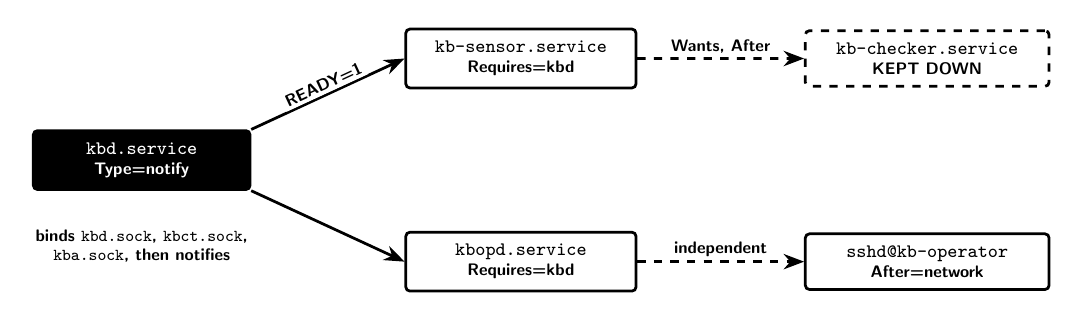
\begin{tikzpicture}[x=1cm,y=1cm,scale=0.86,transform shape]
  \node[dark,minimum width=3.2cm] (kbd) at (0,0) {\unit{kbd.service}\\[-1pt]\scriptsize Type=notify};
  \node[box,minimum width=3.4cm] (sen) at (5.6,1.5) {\unit{kb-sensor.service}\\[-1pt]\scriptsize Requires=kbd};
  \node[box,minimum width=3.4cm] (opd) at (5.6,-1.5) {\unit{kbopd.service}\\[-1pt]\scriptsize Requires=kbd};
  \node[dashedbox,minimum width=3.6cm] (chk) at (11.6,1.5) {\unit{kb-checker.service}\\[-1pt]\scriptsize KEPT DOWN};
  \node[box,minimum width=3.6cm] (ssh) at (11.6,-1.5) {\unit{sshd@kb-operator}\\[-1pt]\scriptsize After=network};
  \draw[flow] (kbd.north east) -- node[lbl,above,sloped]{READY=1} (sen.west);
  \draw[flow] (kbd.south east) -- (opd.west);
  \draw[flowd] (sen) -- node[lbl,above]{Wants, After} (chk);
  \draw[flowd] (opd) -- node[lbl,above]{independent} (ssh);
  \node[font=\bfseries\sffamily\scriptsize,anchor=north,align=center] at (0,-0.9) {binds \texttt{kbd.sock}, \texttt{kbct.sock},\\\texttt{kba.sock}, then notifies};
\end{tikzpicture}
\caption{Start order. \texttt{kbd} sends \texttt{sd\_notify(READY=1)} only after its sockets exist, so
the units that \texttt{Require} it never race ahead of it. The dashed box is the unit held down by the
maintenance condition.}
\end{figure}

\begin{center}\small
\begin{tabularx}{\textwidth}{@{}L{3.3cm}L{3.2cm}Y@{}}
\toprule
\textbf{Unit} & \textbf{Runs} & \textbf{Notes}\\
\midrule
\unit{kbd.service} & \cmd{kbd} with \texttt{--db} \file{/var/lib/kbd/state.db} and \texttt{--policy}, \texttt{--rules}, \texttt{--workloads} from \file{/etc/kb} & \texttt{Type=notify}; \texttt{RuntimeDirectory=kb}; \texttt{StateDirectory=kbd}; sets \texttt{KB\_HTTP\_CORS\_ORIGIN}; loads \file{/etc/kb/api.env}; after readiness runs \texttt{chgrp kb /run/kb/kba.sock}. Conservative hardening only.\\
\unit{kb-sensor.service} & \cmd{kbd\_sensor} & Root, no capability dropping (needs CAP\_BPF/PERFMON/SYS\_ADMIN). Loads the eBPF hooks; connects to \file{kbd.sock}.\\
\unit{kbopd.service} & \cmd{kbopd} headless & Serves the dashboard on 127.0.0.1:8082 and spawns \cmd{mcp-server}. Fully hardened (\texttt{ProtectSystem=strict}, empty capability set).\\
\unit{sshd@kb-operator.service} & \cmd{sshd -D -f} \file{/etc/kb/sshd_kb-operator.conf} & Dedicated instance on port 2222, key-only, forces the wrapper script. Runs with a minimal capability set (\texttt{CAP\_SYS\_CHROOT}, \texttt{SETUID}, \texttt{SETGID}, \texttt{CHOWN}, \texttt{KILL}, \texttt{AUDIT\_WRITE}); an empty set breaks sshd's privilege separation.\\
\unit{kb-checker.service} & \cmd{kb-checker monitor --all} & \textbf{Held down}: never enabled or auto-started; runs only if you start it by hand.\\
\unit{kbagents.service} & \cmd{kbagents} & Installed, not enabled; see Chapter~\ref{ch:aads}.\\
\bottomrule
\end{tabularx}
\end{center}

\section{The one-command start}
\resetsteps
\step{Authorize your SSH public key first (once)}
\begin{lstlisting}[style=console]
$ sudo kbctl ssh add-key ~/.ssh/id_ed25519.pub
key authorized for operator
\end{lstlisting}
\step{Bring the stack up}
\begin{lstlisting}[style=console]
$ sudo kbctl up
\end{lstlisting}
This runs \texttt{systemctl enable --now kbd.service kb-sensor.service kbopd.service sshd@kb-operator.service}
in that order. \cmd{kbctl} adds \texttt{sudo} itself when you are not root, so plain \texttt{kbctl up} also works
and prompts for your password.
\step{Confirm}
\begin{lstlisting}[style=console]
$ kbctl status
kbd.service                  active
kb-sensor.service            active
kbopd.service                active
sshd@kb-operator.service     active
kb-checker.service           UNDER MAINTENANCE AND REPAIRS (kept down)
\end{lstlisting}
\step{Open a surface}
\begin{lstlisting}[style=console]
$ kbctl dashboard open        # web, http://127.0.0.1:8082
$ kbctl ssh connect           # TUI over the operator sshd
$ kbctl tui                   # TUI directly on this terminal
\end{lstlisting}

\section{The same thing with \cmd{systemctl}}
Every \cmd{kbctl} verb is a thin wrapper. Know the equivalents; they are what you use when \cmd{kbd} is down
and \cmd{kbctl} cannot dial it.
\begin{center}\small
\begin{tabularx}{\textwidth}{@{}L{4.6cm}Y@{}}
\toprule
\textbf{kbctl} & \textbf{systemctl equivalent}\\
\midrule
\texttt{kbctl up} & \texttt{systemctl enable --now kbd kb-sensor kbopd sshd@kb-operator}\\
\texttt{kbctl down} & \texttt{systemctl stop} on those four, in reverse order (does not disable)\\
\texttt{kbctl status} & \texttt{systemctl is-active} on each unit, plus the maintenance label\\
\texttt{kbctl dashboard up / down} & \texttt{systemctl enable --now / disable --now kbopd}\\
\texttt{kbctl ssh up / down} & \texttt{systemctl enable --now / disable --now sshd@kb-operator}\\
\bottomrule
\end{tabularx}
\end{center}
\begin{kbnote}
\texttt{up} \emph{enables} units (they start at every boot). \texttt{down} only \emph{stops} the whole stack and
leaves it enabled, so a reboot brings it back. To keep a unit down across reboots use
\texttt{kbctl dashboard down} or \texttt{kbctl ssh down}, which also \emph{disable} it.
\end{kbnote}

\section{Watching a start succeed}
\begin{lstlisting}[style=console]
$ journalctl -u kbd -u kb-sensor -u kbopd -f
... kbd: [KB] gRPC health service registered, status=SERVING for "kernel-borderlands"
... kbd: [KB] audit log hash chain verified intact (0 entries)
... kbd: [KB] Control plane ready
... kb-sensor: (6 hooks attached; uprobes into libssl/libgnutls)
... kbopd: Vite Dashboard Server listening on http://localhost:8082
\end{lstlisting}
\texttt{kbd} printing \texttt{audit log hash chain verified intact} on every start is the cheapest tamper check
you will ever get; see Section~\ref{sec:audit}.

\section{Stopping, restarting, and what to expect}
\begin{center}\small
\begin{tabularx}{\textwidth}{@{}L{4.2cm}Y@{}}
\toprule
\textbf{You do} & \textbf{What happens}\\
\midrule
\texttt{sudo systemctl restart kbd} & \texttt{kb-sensor} and \texttt{kbopd} (which \texttt{Require} it) are restarted with it; the sensor reconnects and \cmd{kbd} re-pushes the rules and sensitive paths at connect time.\\
\texttt{sudo systemctl stop kb-sensor} & Telemetry stops; existing containment stays in the kernel maps until cleared. \cmd{kbd} keeps serving history.\\
\texttt{sudo kbctl down} & Orderly stop in reverse boot order.\\
Power loss & \texttt{kbd}'s SQLite WAL replays on next start (\texttt{L1 restored from L2}).\\
\bottomrule
\end{tabularx}
\end{center}

\chapter{The Web Dashboard}
\label{ch:dash}
\section{How it is put together}
\begin{figure}[ht]
\centering
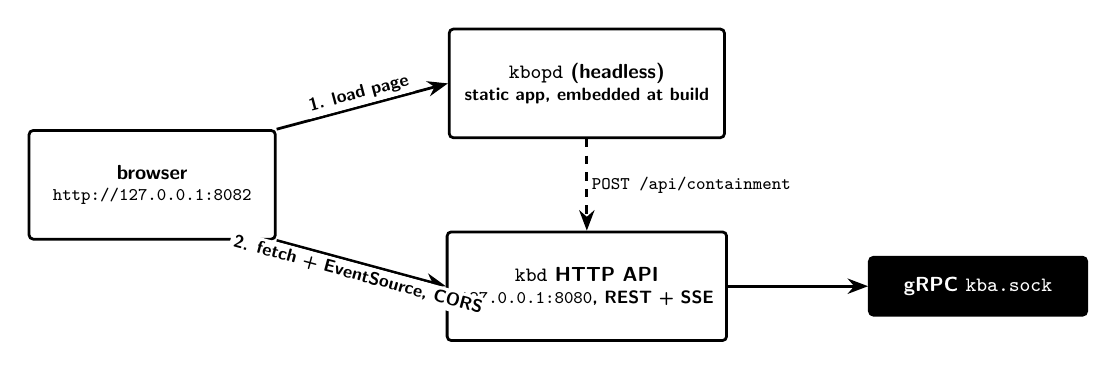
\begin{tikzpicture}[x=1cm,y=1cm,scale=0.92,transform shape]
  \node[box,minimum width=3.4cm,minimum height=1.5cm] (br) at (0,0) {browser\\[-1pt]\scriptsize \texttt{http://127.0.0.1:8082}};
  \node[box,minimum width=3.8cm,minimum height=1.5cm] (opd) at (6,1.4) {\texttt{kbopd} (headless)\\[-1pt]\scriptsize static app, embedded at build};
  \node[box,minimum width=3.8cm,minimum height=1.5cm] (kbd) at (6,-1.4) {\texttt{kbd} HTTP API\\[-1pt]\scriptsize \texttt{127.0.0.1:8080}, REST + SSE};
  \node[dark,minimum width=3cm] (gr) at (11.4,-1.4) {gRPC \texttt{kba.sock}};
  \draw[flow] (br.north east) -- node[lbl,above,sloped]{1. load page} (opd.west);
  \draw[flow] (br.south east) -- node[lbl,below,sloped]{2. fetch + EventSource, CORS} (kbd.west);
  \draw[flow] (kbd) -- (gr);
  \draw[flowd] (opd.south) -- node[lbl,right]{\texttt{POST /api/containment}} (kbd.north);
\end{tikzpicture}
\caption{The page itself comes from \texttt{kbopd} on 8082; every data call goes from the \emph{browser}
straight to \texttt{kbd} on 8080. That second hop is cross-origin and is why \texttt{KB\_HTTP\_CORS\_ORIGIN}
exists.}
\end{figure}
The dashboard's JavaScript builds its API address as \texttt{http://<the host you loaded it from>:8080}.
Loaded via \texttt{127.0.0.1} it calls \texttt{127.0.0.1:8080}; loaded via \texttt{localhost} it calls
\texttt{localhost:8080}. Both origins are in the packaged allowlist; any other hostname is blocked by the
browser until you add it.

\section{Commands}
\begin{lstlisting}[style=console]
$ kbctl dashboard up        # enable + start kbopd, wait for the port, print the URL
dashboard up: http://127.0.0.1:8082
$ kbctl dashboard open      # up (if needed) + launch the default browser
opened http://127.0.0.1:8082
$ kbctl dashboard status    # exit 0 if active AND listening, 3 otherwise
kbopd.service: active, http://127.0.0.1:8082 listening=true
$ kbctl dashboard url       # just print it, handy in scripts
$ kbctl dashboard down      # stop + disable
\end{lstlisting}
\cmd{up} polls the port for up to 15~seconds. If no browser can be launched (a headless server),
\cmd{open} prints the URL and succeeds; open it from another machine through the tunnel below.

\section{Reaching it from your workstation}
The dashboard binds loopback only. The operator \cmd{sshd} deliberately forbids TCP forwarding
(\texttt{AllowTcpForwarding no}), so tunnel through your \emph{normal} SSH service (port 22):
\begin{lstlisting}[style=console]
workstation$ ssh -N -L 8082:127.0.0.1:8082 -L 8080:127.0.0.1:8080 you@kb-host
workstation$ xdg-open http://127.0.0.1:8082
\end{lstlisting}
Forward \emph{both} ports: the page comes from 8082, the data from 8080. Use \texttt{127.0.0.1} (or
\texttt{localhost}) in the browser, matching the CORS allowlist.

\section{What the API exposes}
\begin{center}\small
\begin{tabularx}{\textwidth}{@{}L{4.2cm}L{1.6cm}Y@{}}
\toprule
\textbf{Route on \texttt{:8080}} & \textbf{Auth} & \textbf{Purpose}\\
\midrule
\texttt{/api/processes} & none & Tracked processes and zones.\\
\texttt{/api/alerts}, \texttt{/api/logs} & none & Alert stream snapshot, log tail.\\
\texttt{/api/services} & none & Health of KB services.\\
\texttt{/api/metrics} & none & Event rates, active process counts.\\
\texttt{/api/agents} & none & Proxied from the swarm status server (:8601).\\
\texttt{/api/policy} & none & Current policy.\\
\texttt{/api/audit/verify} & none & Hash-chain verification.\\
\texttt{/api/events} & none & Server-Sent Events live stream.\\
\texttt{/api/isolate}, \texttt{/api/restore} & \textbf{token} & Contain / release a process.\\
\texttt{/api/policy/reload} & \textbf{token} & Reload \file{policy.yaml}.\\
\bottomrule
\end{tabularx}
\end{center}
\begin{kbwarn}[THE ACTION BUTTONS NEED A TOKEN]
The three mutating routes are wrapped in \texttt{requireAPIToken} and \textbf{fail closed}: with no
\texttt{KB\_HTTP\_API\_TOKEN} configured they are unusable, not unauthenticated. The read-only views work out
of the box; to use isolate, restore or policy-reload from the browser, set a token with a drop-in
(Section~\ref{sec:dropin}) and supply it as the dashboard expects. Until then use \cmd{kbctl}, which talks gRPC
over the root-only socket and needs no token.
\end{kbwarn}

\section{Symptoms and causes}
\begin{center}\small
\begin{tabularx}{\textwidth}{@{}L{4.4cm}Y@{}}
\toprule
\textbf{You see} & \textbf{Cause and fix}\\
\midrule
Page loads, every panel empty, console shows CORS errors & The page's origin is not in \texttt{KB\_HTTP\_CORS\_ORIGIN}. Load via \texttt{127.0.0.1} or \texttt{localhost}, or add your origin in a drop-in and restart \cmd{kbd}.\\
\texttt{connection refused} on 8082 & \unit{kbopd.service} is not running: \texttt{kbctl dashboard status}.\\
Page loads but data source shows a different host & You loaded it via a hostname not in the allowlist; the dashboard derives the API host from the page URL.\\
\texttt{kbctl dashboard up} times out & \texttt{journalctl -u kbopd}. Another process already holds 8082.\\
\bottomrule
\end{tabularx}
\end{center}

\chapter{The SSH Terminal Console}
\label{ch:ssh}
\section{The architecture}
The console is not a feature of \cmd{kbd}. It is a \emph{second, independent} \cmd{sshd} that exists only to
authenticate an operator and force one program. Host keys, \file{authorized_keys} and PTY handling all live
in that \cmd{sshd}.

\begin{figure}[ht]
\centering
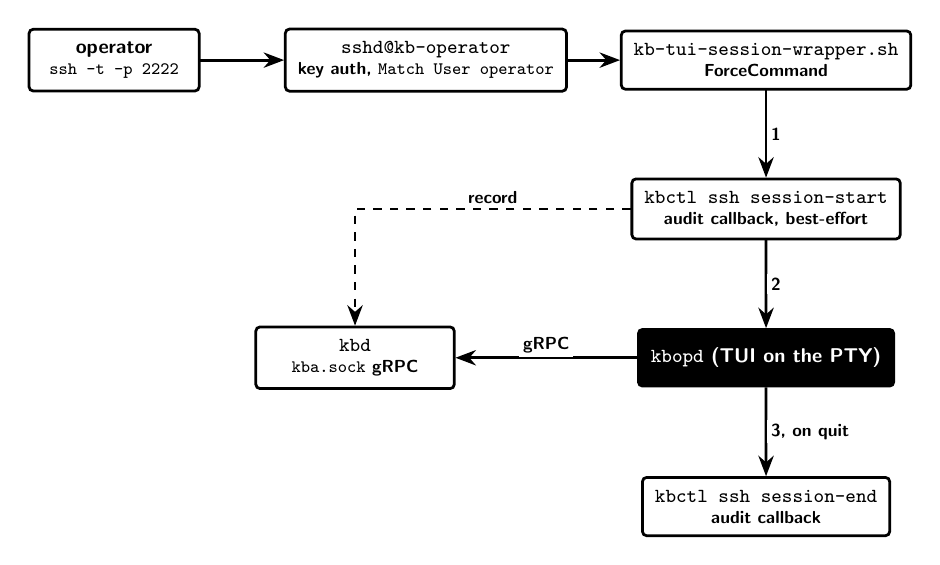
\begin{tikzpicture}[x=1cm,y=1cm,scale=0.9,transform shape]
  \node[box,minimum width=2.4cm] (cl) at (0,0) {operator\\[-1pt]\scriptsize \texttt{ssh -t -p 2222}};
  \node[box,minimum width=3.2cm] (sd) at (4.4,0) {\texttt{sshd@kb-operator}\\[-1pt]\scriptsize key auth, \texttt{Match User operator}};
  \node[box,minimum width=3.6cm] (wr) at (9.2,0) {\texttt{kb-tui-session-wrapper.sh}\\[-1pt]\scriptsize ForceCommand};
  \node[box,minimum width=3.2cm] (s1) at (9.2,-2.1) {\texttt{kbctl ssh session-start}\\[-1pt]\scriptsize audit callback, best-effort};
  \node[dark,minimum width=3.2cm] (tui) at (9.2,-4.2) {\texttt{kbopd} (TUI on the PTY)};
  \node[box,minimum width=3.2cm] (s2) at (9.2,-6.3) {\texttt{kbctl ssh session-end}\\[-1pt]\scriptsize audit callback};
  \node[box,minimum width=2.8cm] (kbd) at (3.4,-4.2) {\texttt{kbd}\\[-1pt]\scriptsize \texttt{kba.sock} gRPC};
  \draw[flow] (cl) -- (sd); \draw[flow] (sd) -- (wr);
  \draw[flow] (wr) -- node[lbl,right]{1} (s1); \draw[flow] (s1) -- node[lbl,right]{2} (tui);
  \draw[flow] (tui) -- node[lbl,right]{3, on quit} (s2);
  \draw[flow] (tui) -- node[lbl,above]{gRPC} (kbd);
  \draw[flowd] (s1.west) -| node[lbl,pos=0.25,above]{record} (kbd.north);
\end{tikzpicture}
\caption{One SSH session. The wrapper records the start, runs the TUI, records the end, and returns the
TUI's exit status to the client.}
\end{figure}
Both audit callbacks are \textbf{best-effort by design}. If \cmd{kbd} is down, \cmd{kbctl ssh session-start}
prints a warning to the operator's terminal and exits 0; an audit-logging outage must never become a denial of
access to the very tool you need during an incident.

\section{Commands}
\begin{lstlisting}[style=console]
$ sudo kbctl ssh up            # enable + start sshd@kb-operator, wait for :2222
$ kbctl ssh status             # exit 0 only if active AND port answering
$ sudo kbctl ssh add-key ~/.ssh/id_ed25519.pub
key authorized for operator
$ kbctl ssh connect            # to 127.0.0.1:2222 as operator, starting it if needed
$ kbctl ssh connect kb-host    # to a remote host
$ kbctl ssh connect kb-host -i ~/.ssh/ops_key --port 2222
$ sudo kbctl ssh down          # stop + disable
\end{lstlisting}
\cmd{ssh connect} replaces itself with \cmd{ssh -t} (so your terminal, window resizes and exit status are
real SSH's). For loopback targets it adds \texttt{UserKnownHostsFile=/dev/null} and
\texttt{StrictHostKeyChecking=no}, because the host key is regenerated per machine and would otherwise
pollute \file{known_hosts}; \emph{remote} hosts keep normal host-key checking.

\subsection{\cmd{add-key} in detail}
It accepts a public-key file or \texttt{-} for stdin, requires \textbf{exactly one line}, checks the key type
prefix (\texttt{ssh-ed25519}, \texttt{ssh-rsa}, \texttt{ecdsa-sha2-*}, \texttt{sk-*}), skips a key already present,
and appends to \file{/etc/kb/authorized_keys} with \cmd{tee -a} under \cmd{sudo} (the file is \texttt{operator:kb} 0600).
\begin{lstlisting}[style=console]
$ ssh-add -L | head -1 | sudo kbctl ssh add-key -     # from an agent
$ printf 'garbage\n' | kbctl ssh add-key -
error: not an OpenSSH public key (want ssh-ed25519/ecdsa-sha2-*/sk-*/ssh-rsa ...)
\end{lstlisting}

\section{The sshd configuration, line by line}
\lstinputlisting[style=conf,caption={\file{/etc/kb/sshd_kb-operator.conf} (packaged)}]{../../packaging/ssh/kb-operator.conf}
\begin{center}\small
\begin{tabularx}{\textwidth}{@{}L{4.6cm}Y@{}}
\toprule
\textbf{Directive} & \textbf{Effect}\\
\midrule
\texttt{Port 2222} & Dedicated port, separate from the host's port 22.\\
\texttt{HostKey /etc/kb/ssh/...} & Host key private to this instance.\\
\texttt{Match User operator} & Everything below applies only to the \texttt{operator} account.\\
\texttt{ForceCommand ...wrapper.sh} & Whatever the client asks to run, this runs instead.\\
\texttt{AuthorizedKeysFile /etc/kb/authorized\_keys} & Keys live outside any home directory.\\
\texttt{X11Forwarding no}, \texttt{AllowTcpForwarding no} & No tunnels through the console.\\
\texttt{PermitTTY yes} & The TUI needs a PTY.\\
\bottomrule
\end{tabularx}
\end{center}
\begin{kbnote}[HARDENING YOU MAY WANT TO ADD]
The packaged file does not disable password authentication for non-\texttt{operator} users. The
\texttt{operator} account has no password, so it is moot for that account, but adding
\texttt{PasswordAuthentication no} and \texttt{KbdInteractiveAuthentication no} makes the whole instance
key-only. Edit \file{/etc/kb/sshd_kb-operator.conf}; it is a protected config file and survives upgrades.
\end{kbnote}

\section{Check the console on your host}
\label{sec:nologin}
OpenSSH runs a \texttt{ForceCommand} through the account's login shell, which a \texttt{nologin} shell refuses.
\file{provision.sh} therefore creates \texttt{operator} with \file{/bin/sh}, and the package's migration step fixes an
existing account that still has \texttt{nologin} or \texttt{false}. This has \textbf{not} been exercised on a live host (no root in
the build sessions), so run this check once after \cmd{kbctl up}:
\resetsteps
\step{Connect}
\begin{lstlisting}[style=console]
$ kbctl ssh connect
\end{lstlisting}
\step{Read the result}
\begin{itemize}
\item \textbf{The TUI appears.} Nothing to do.
\item \textbf{``This account is currently not available.''} and the connection closes: the account still has a \texttt{nologin} shell (for example the package was installed before this fix and the migration did not run). Fix it as below.
\end{itemize}
\step{If refused, give the account a plain shell by hand}
\begin{lstlisting}[style=console]
$ sudo usermod --shell /bin/sh operator
$ kbctl ssh connect
\end{lstlisting}
This is safe in this design: the only way in is a key in \file{/etc/kb/authorized_keys}, the config forces
the wrapper and forbids forwarding, and the account has no password.

\section{Using the TUI}
\subsection{The four tabs}
\texttt{Tab} moves forward, \texttt{Shift+Tab} backward. \texttt{?} toggles help (\texttt{Esc} also closes it).
\texttt{q} or \texttt{Ctrl+C} quits.
\begin{center}\small
\begin{tabularx}{\textwidth}{@{}L{3cm}L{4.2cm}Y@{}}
\toprule
\textbf{Tab} & \textbf{Keys} & \textbf{Meaning}\\
\midrule
Processes & \texttt{j}/\texttt{k} or arrows & Move selection through the process table (PID, COMM, ZONE, SCORE, UID, CONTAINMENT).\\
 & \texttt{/} & Start a filter; type to narrow, \texttt{Enter}/\texttt{Esc} to stop typing, \texttt{Esc} again clears it.\\
 & \texttt{c} & Contain the selected process (see below).\\
Alerts & \texttt{j}/\texttt{k}, \texttt{Enter} & Scroll alerts; \texttt{Enter} expands or collapses one.\\
Agent Activity & \texttt{j}/\texttt{k} & Scroll the swarm's activity feed.\\
Query Console & type, \texttt{Enter} & Run a command; \texttt{Up}/\texttt{Down} history; \texttt{Ctrl+U} clears the line.\\
\bottomrule
\end{tabularx}
\end{center}

\subsection{Containing a process}
\resetsteps
\step{Select it and press \texttt{c}.} A modal asks for a level.
\step{Pick the level.}
\begin{center}\small
\begin{tabular}{@{}ll@{}}
\toprule \textbf{Key} & \textbf{Level}\\ \midrule
\texttt{0} & None (release)\\ \texttt{1} & Cgroup\\ \texttt{2} & Seccomp\\ \texttt{3} & Namespace\\ \texttt{4} & Terminate\\ \bottomrule
\end{tabular}
\end{center}
\step{Confirm.} \texttt{y} or \texttt{Enter} submits with the reason \texttt{operator action via kb-tui};
\texttt{n} returns to level selection; \texttt{Esc} cancels.

\subsection{The query console}
\begin{lstlisting}[style=console]
> help
> pid 4242                      # full state for one process
> zone borderlands              # list processes in safe|suspicious|borderlands
> stats                         # global telemetry snapshot
> contain 4242 seccomp suspicious beaconing
> clear
\end{lstlisting}
Levels for \texttt{contain}: \texttt{none, cgroup, seccomp, namespace, terminate}.

\subsection{When \cmd{kbd} is unreachable}
If \file{/run/kb/kba.sock} cannot be dialed the TUI does \emph{not} fail. It shows an
\texttt{[OFFLINE]} banner (``\texttt{kbd unreachable}'') and a \texttt{[DEMO DATA]} table so you can see the
interface working. Never act on demo rows: the PIDs are fictional. Read the banner before the table.

\chapter{kbctl Reference}
\label{ch:kbctl}
\cmd{kbctl} is the programmatic workhorse. Every control operation is a typed protobuf gRPC request over
\file{/run/kb/kba.sock}. The reference text below is \textbf{generated from the installed binary's
\texttt{--help}} by \file{latex/field-manual/gen-help.sh}, so it cannot drift from the code.

\newcommand{\helpblock}[2]{\subsection{#1}\lstinputlisting[style=console]{generated/kbctl-#2.txt}}

\section{Command map}
\begin{figure}[ht]
\centering
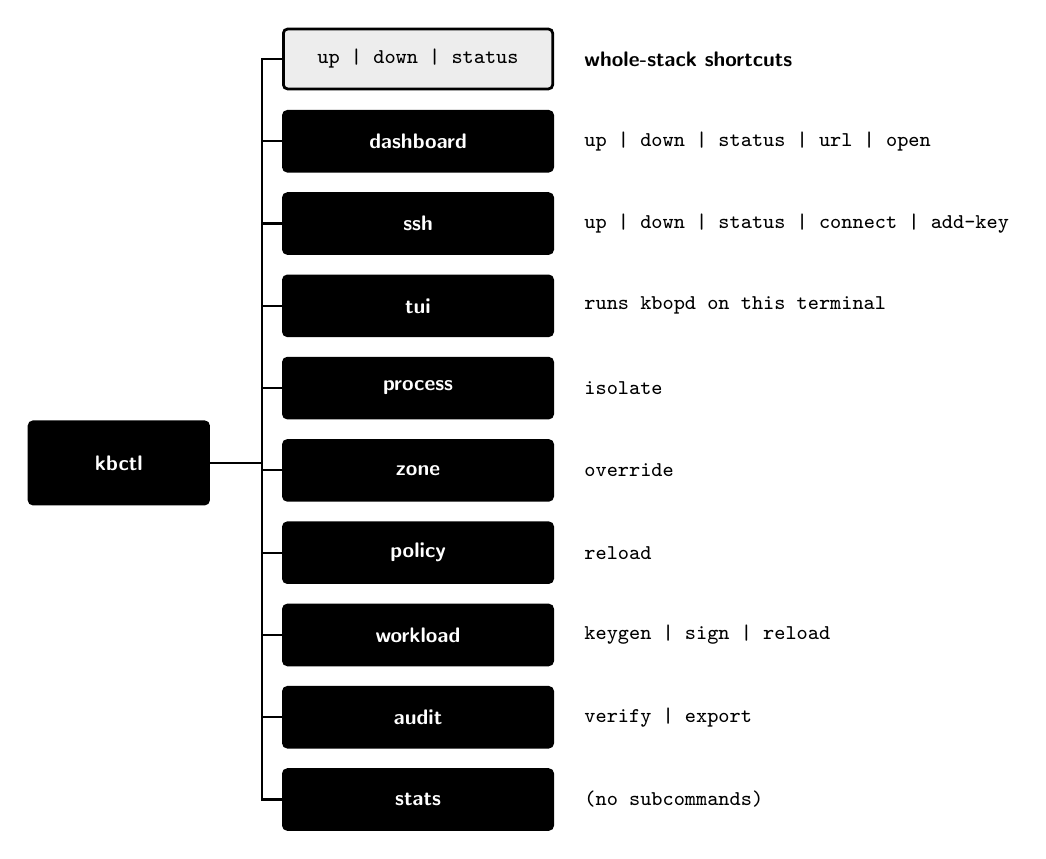
\begin{tikzpicture}[x=1cm,y=1cm,scale=0.95,transform shape]
  \node[dark,minimum width=2.4cm,minimum height=1.1cm] (root) at (0,-5.4) {kbctl};
  \node[soft,minimum width=3.6cm] (g0) at (4,-0.0) {\texttt{up | down | status}};
  \node[anchor=west,font=\bfseries\sffamily\footnotesize] at (6.1,-0.0) {whole-stack shortcuts};
  \node[dark,minimum width=3.6cm] (g1) at (4,-1.1) {dashboard};
  \node[anchor=west,font=\ttfamily\bfseries\footnotesize] at (6.1,-1.1) {up | down | status | url | open};
  \node[dark,minimum width=3.6cm] (g2) at (4,-2.2) {ssh};
  \node[anchor=west,font=\ttfamily\bfseries\footnotesize] at (6.1,-2.2) {up | down | status | connect | add-key};
  \node[dark,minimum width=3.6cm] (g3) at (4,-3.3000000000000003) {tui};
  \node[anchor=west,font=\ttfamily\bfseries\footnotesize] at (6.1,-3.3000000000000003) {runs kbopd on this terminal};
  \node[dark,minimum width=3.6cm] (g4) at (4,-4.4) {process};
  \node[anchor=west,font=\ttfamily\bfseries\footnotesize] at (6.1,-4.4) {isolate};
  \node[dark,minimum width=3.6cm] (g5) at (4,-5.5) {zone};
  \node[anchor=west,font=\ttfamily\bfseries\footnotesize] at (6.1,-5.5) {override};
  \node[dark,minimum width=3.6cm] (g6) at (4,-6.6000000000000005) {policy};
  \node[anchor=west,font=\ttfamily\bfseries\footnotesize] at (6.1,-6.6000000000000005) {reload};
  \node[dark,minimum width=3.6cm] (g7) at (4,-7.700000000000001) {workload};
  \node[anchor=west,font=\ttfamily\bfseries\footnotesize] at (6.1,-7.700000000000001) {keygen | sign | reload};
  \node[dark,minimum width=3.6cm] (g8) at (4,-8.8) {audit};
  \node[anchor=west,font=\ttfamily\bfseries\footnotesize] at (6.1,-8.8) {verify | export};
  \node[dark,minimum width=3.6cm] (g9) at (4,-9.9) {stats};
  \node[anchor=west,font=\ttfamily\bfseries\footnotesize] at (6.1,-9.9) {(no subcommands)};
  \foreach \i in {0,...,9} \draw[line width=0.8pt] (root.east) -- ++(0.7,0) |- (g\i.west);
\end{tikzpicture}
\caption{Everything under \texttt{kbctl}. The first row are top-level shortcuts that act on the whole stack.}
\end{figure}

\section{Global flag}
\begin{lstlisting}[style=console]
--socket string   path to kbd's gRPC Unix domain socket (default "/run/kb/kba.sock")
\end{lstlisting}
Only commands that talk to \cmd{kbd} use it (\texttt{policy}, \texttt{workload reload}, \texttt{zone},
\texttt{process}, \texttt{audit}, \texttt{stats}). The service-control commands (\texttt{up}, \texttt{down},
\texttt{status}, \texttt{dashboard}, \texttt{ssh}) go through \cmd{systemctl} and work even when \cmd{kbd} is down.

\section{Exit codes}
\begin{center}\small
\begin{tabularx}{\textwidth}{@{}L{1.6cm}Y@{}}
\toprule
\textbf{Code} & \textbf{Meaning}\\
\midrule
0 & Success. For \texttt{dashboard status} and \texttt{ssh status}: the unit is active \emph{and} the port answers.\\
1 & Error (printed as \texttt{error: ...}): bad arguments, RPC failure, \texttt{systemctl} failure.\\
3 & \texttt{dashboard status} / \texttt{ssh status} only: unit not active or port not listening. Use it in scripts.\\
\bottomrule
\end{tabularx}
\end{center}

\section{Stack control}
\helpblock{kbctl up}{up}
\helpblock{kbctl down}{down}
\helpblock{kbctl status}{status}

\section{Web dashboard}
\helpblock{kbctl dashboard}{dashboard}
\helpblock{kbctl dashboard open}{dashboard-open}
\helpblock{kbctl dashboard status}{dashboard-status}
\helpblock{kbctl dashboard url}{dashboard-url}

\section{SSH console and TUI}
\helpblock{kbctl ssh}{ssh}
\helpblock{kbctl ssh connect}{ssh-connect}
\helpblock{kbctl ssh add-key}{ssh-add-key}
\helpblock{kbctl tui}{tui}

\section{Containment and classification}
\helpblock{kbctl process isolate}{process-isolate}
\textbf{Levels} are \texttt{CGROUP}, \texttt{SECCOMP}, \texttt{NAMESPACE} (default) and \texttt{TERMINATE}, in
increasing severity. The command prints \texttt{pid=N contained at level L}. The reason is written to the audit log.
\helpblock{kbctl zone override}{zone-override}
\begin{kbnote}[OVERRIDE IS COSMETIC, NOT ENFORCEMENT]
\texttt{zone override} relabels how \cmd{kbd} \emph{displays and classifies} a process. It does not touch
kernel or enforcement state, and the next real zone transition from the sensor overwrites it. To actually
restrict a process, use \texttt{process isolate}.
\end{kbnote}

\section{Policy, workloads, audit, stats}
\helpblock{kbctl policy reload}{policy-reload}
\helpblock{kbctl workload keygen}{workload-keygen}
\helpblock{kbctl workload sign}{workload-sign}
\helpblock{kbctl workload reload}{workload-reload}
\helpblock{kbctl audit verify}{audit-verify}
\helpblock{kbctl audit export}{audit-export}
\helpblock{kbctl stats}{stats}

\section{The daemons' own flags}
\subsection{kbd}
\lstinputlisting[style=console]{generated/kbd.txt}
\subsection{kb-checker (kept down; for reference)}
\lstinputlisting[style=console]{generated/kb-checker-monitor.txt}

\chapter{Command Combinations and Playbooks}
\label{ch:play}
A command is a word; a playbook is a sentence. Each recipe below is complete, ordered, and says what you
should see after every step.

\section{Playbook 1: cold start to first dashboard}
\begin{lstlisting}[style=console]
$ sudo kbctl ssh add-key ~/.ssh/id_ed25519.pub     # once per operator
$ sudo kbctl up
$ kbctl status                                      # all four active
$ kbctl dashboard open                              # browser appears
$ kbctl stats
events/sec:       112.40
active processes: 238
\end{lstlisting}
If \texttt{stats} errors with \texttt{dial unix /run/kb/kba.sock: no such file}, \cmd{kbd} is not running:
\texttt{systemctl status kbd}.

\section{Playbook 2: a remote operator takes over}
On the server (once): \texttt{sudo kbctl ssh add-key} for their key, \texttt{sudo kbctl ssh up}.
On their laptop:
\begin{lstlisting}[style=console]
$ ssh -t -p 2222 operator@kb-host        # lands directly in the TUI, nothing else
\end{lstlisting}
They need no account on the server and get no shell. Revoke by deleting their line from
\file{/etc/kb/authorized_keys}; no restart is needed.

\section{Playbook 3: incident, from detection to containment}
\begin{figure}[ht]
\centering
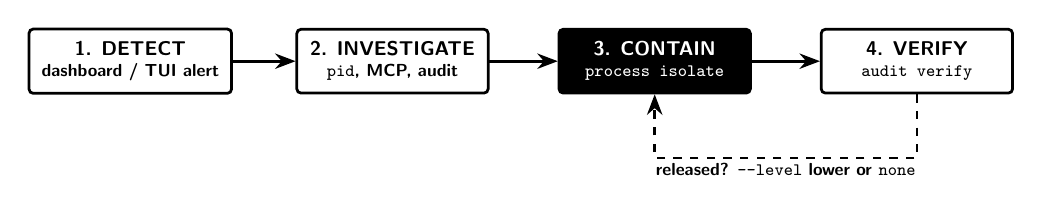
\begin{tikzpicture}[x=1cm,y=1cm,scale=0.9,transform shape]
  \node[box,minimum width=2.7cm] (d) at (0,0) {1. DETECT\\[-1pt]\scriptsize dashboard / TUI alert};
  \node[box,minimum width=2.7cm] (i) at (3.7,0) {2. INVESTIGATE\\[-1pt]\scriptsize \texttt{pid}, MCP, audit};
  \node[dark,minimum width=2.7cm] (c) at (7.4,0) {3. CONTAIN\\[-1pt]\scriptsize \texttt{process isolate}};
  \node[box,minimum width=2.7cm] (v) at (11.1,0) {4. VERIFY\\[-1pt]\scriptsize \texttt{audit verify}};
  \draw[flow] (d)--(i); \draw[flow] (i)--(c); \draw[flow] (c)--(v);
  \draw[flowd] (v.south) -- ++(0,-0.9) -| node[lbl,pos=0.25,below]{released? \texttt{--level} lower or \texttt{none}} (c.south);
\end{tikzpicture}
\caption{The response loop. Containment is reversible until you choose \texttt{TERMINATE}.}
\end{figure}
\resetsteps
\step{Detect.} A process enters \texttt{BORDERLANDS}. The dashboard raises a \texttt{BORDERLANDS\_ENTRY} alert.
\step{Investigate.} In the TUI Query Console: \texttt{pid 4242}, \texttt{zone borderlands}.
\step{Contain, mildest effective level first.}
\begin{lstlisting}[style=console]
$ sudo kbctl process isolate --pid 4242 --level SECCOMP \
      --reason "beaconing to unknown ASN, ticket 1187"
pid=4242 contained at level SECCOMP
\end{lstlisting}
Escalate to \texttt{NAMESPACE} only if the behaviour continues; reserve \texttt{TERMINATE} for confirmed hostile code.
\step{Verify the record.}
\begin{lstlisting}[style=console]
$ kbctl audit verify
chain intact — 1432 entries verified     # counts will differ
\end{lstlisting}

\section{Playbook 4: change policy without restarting}
\label{sec:policy-change}
\begin{lstlisting}[style=console]
$ sudo $EDITOR /etc/kb/policy.yaml
$ sudo kbctl policy reload
\end{lstlisting}
\cmd{kbd} re-reads the file it was \emph{started with} (\file{/etc/kb/policy.yaml} in the packaged unit) and
logs how many process policies and extra sensitive paths it loaded.

\section{Playbook 5: protect a workload with signed CWP rules}
\label{sec:cwp}
Protected-workload rules can require a signature so nobody can weaken them by editing a file.
\resetsteps
\step{Create a signing key pair somewhere safe (not on the monitored host if you can avoid it).}
\begin{lstlisting}[style=console]
$ kbctl workload keygen --out-dir ~/kb-keys --name cwp-signer
Wrote private key (keep secret): /home/you/kb-keys/cwp-signer.key
Wrote public key (for kbd's --workloads-pubkey): /home/you/kb-keys/cwp-signer.pub
\end{lstlisting}
\step{Edit and sign. The file is rewritten \emph{in place}.}
\begin{lstlisting}[style=console]
$ sudo $EDITOR /etc/kb/workloads.yaml
$ sudo kbctl workload sign /etc/kb/workloads.yaml \
      --key ~/kb-keys/cwp-signer.key --signed-by "alice@soc" --version 2
Signed /etc/kb/workloads.yaml (signed_by="alice@soc" version=2)
\end{lstlisting}
\step{Tell \cmd{kbd} to require the signature.} Install the public key and add a drop-in (Section~\ref{sec:dropin}):
\begin{lstlisting}[style=console]
$ sudo install -m644 ~/kb-keys/cwp-signer.pub /etc/kb/workloads.pub
$ sudo systemctl edit kbd
[Service]
ExecStart=
ExecStart=/usr/bin/kbd --db /var/lib/kbd/state.db --policy /etc/kb/policy.yaml \
    --rules /etc/kb/rules.yaml --workloads /etc/kb/workloads.yaml \
    --workloads-pubkey /etc/kb/workloads.pub
$ sudo systemctl restart kbd
\end{lstlisting}
\step{Push live to every connected sensor.}
\begin{lstlisting}[style=console]
$ sudo kbctl workload reload
\end{lstlisting}
Without \texttt{--workloads-pubkey}, CWP stays unsigned and opt-in; an unsigned file is accepted.

\section{Playbook 6: prove the audit log is intact}
\label{sec:audit}
\begin{lstlisting}[style=console]
$ kbctl audit verify
chain intact — 1432 entries verified           # counts will differ; exit 0
$ kbctl audit export --out /tmp/audit-$(date +%F).json
wrote 1432 entries to /tmp/audit-2026-10-27.json
\end{lstlisting}
Each entry hashes the previous one (SHA-256). A broken chain prints
\texttt{CHAIN BROKEN — N entries verified before break}. Export before you investigate a suspected break so
you hold a copy of the evidence.

\section{Playbook 7: scripting and health gates}
\begin{lstlisting}[style=console]
# wait until the SSH console really answers, then continue
$ until kbctl ssh status >/dev/null; do sleep 1; done

# fail a CI step if the dashboard is not serving
$ kbctl dashboard status || { echo "dashboard down"; exit 1; }

# watch the stack
$ watch -n2 kbctl status

# stop everything for maintenance, start it again
$ sudo kbctl down && sudo kbctl up

# one-liner health report
$ kbctl status; kbctl stats; kbctl audit verify
\end{lstlisting}
Exit code 3 from the two \texttt{status} commands means ``not up''; code 1 means the command itself failed.

\section{Playbook 8: a quick demo for an audience}
\begin{lstlisting}[style=console]
$ sudo kbctl up
$ kbctl dashboard open                       # screen 1: live dashboard
$ kbctl ssh connect                          # screen 2: the same data in a terminal
# in the TUI: Tab to Processes, press / to filter, c to contain a demo process
$ kbctl audit verify                         # screen 3: the audit proof
\end{lstlisting}
Remember the TUI's \texttt{[DEMO DATA]} banner when \cmd{kbd} is down: do not present fictional rows as live.

\section{Combination cheat sheet}
\begin{center}\small
\begin{tabularx}{\textwidth}{@{}L{5.6cm}Y@{}}
\toprule
\textbf{Goal} & \textbf{Command}\\
\midrule
Everything up and verified & \texttt{sudo kbctl up \&\& kbctl status}\\
Web only & \texttt{kbctl dashboard open}\\
TUI only, on this box & \texttt{kbctl tui}\\
TUI over SSH, loopback & \texttt{kbctl ssh connect}\\
TUI over SSH, remote & \texttt{kbctl ssh connect HOST -i KEY}\\
Add an operator & \texttt{sudo kbctl ssh add-key KEY.pub}\\
Contain, then prove it & \texttt{kbctl process isolate ... \&\& kbctl audit verify}\\
Policy edit, apply & \texttt{sudo \$EDITOR /etc/kb/policy.yaml \&\& sudo kbctl policy reload}\\
Evidence copy & \texttt{kbctl audit export --out FILE}\\
Stop for maintenance & \texttt{sudo kbctl down}\\
Stop one surface permanently & \texttt{kbctl dashboard down} / \texttt{sudo kbctl ssh down}\\
\bottomrule
\end{tabularx}
\end{center}

\chapter{kb-checker: Under Maintenance and Repairs}
\label{ch:checker}
\begin{kbwarn}[STATUS: DOWN, BY DECISION]
\cmd{kb-checker} is \textbf{under maintenance and repairs} and is kept down. This is deliberate and
enforced in three places, so that no one starts it by accident.
\end{kbwarn}

\section{How it is held down}
\begin{center}\small
\begin{tabularx}{\textwidth}{@{}L{4.6cm}Y@{}}
\toprule
\textbf{Mechanism} & \textbf{Effect}\\
\midrule
\file{ConditionPathExists=/etc/kb/checker.enabled} in \unit{kb-checker.service} & \texttt{systemctl start kb-checker} is a no-op that reports the condition failed, until that file exists. The package never creates it.\\
\cmd{kbctl up} & Starts \texttt{kbd}, \texttt{kb-sensor}, \texttt{kbopd}, \texttt{sshd@kb-operator} only.\\
\cmd{kbctl status} & Prints \texttt{UNDER MAINTENANCE AND REPAIRS (kept down)} instead of a state.\\
\unit{kbagents.service} & No longer \texttt{Requires=} the checker, which would have started it.\\
\texttt{packaging/install.sh} & No longer enables it.\\
\bottomrule
\end{tabularx}
\end{center}
\begin{lstlisting}[style=console]
$ sudo systemctl start kb-checker
$ systemctl status kb-checker | grep -E 'Active|Condition'
   Active: inactive (dead)
  Condition: start condition unmet ... ConditionPathExists=/etc/kb/checker.enabled was not met
\end{lstlisting}

\section{What you lose while it is down}
\cmd{kb-checker} audits eBPF bytecode and map integrity, sensor liveness, the \cmd{kbd} gRPC health, and the swarm.
It also runs the \emph{Tampering Containment Protocol}: on a confirmed integrity violation it stops the sensor,
detaches the eBPF links and quarantines the host's network. With it down:
\begin{itemize}
\item \textbf{No automatic tamper response.} Nothing independently notices if the sensor or its programs are altered. Treat the host as \emph{observed but not self-defending}.
\item \textbf{No false lockdowns either.} The checker's fail-closed behaviour can isolate a host over a missing dependency (for example, an absent swarm). Its absence removes that risk during demos.
\item \texttt{/api/services} in the dashboard will report the checker as down. That is expected, not a fault.
\end{itemize}

\begin{kbwarn}[DO NOT RE-ENABLE IT AS A WORKAROUND]
Creating \file{/etc/kb/checker.enabled} arms a component that can kill the sensor and firewall the host. Do it
only on a machine you can reach out-of-band, and only once the repairs are signed off. When they are,
remove the \texttt{ConditionPathExists} line from \file{packaging/systemd/kb-checker.service}, delete the
\texttt{maintenanceUnits} entry in \file{kb-op/kbctl/svc.go}, add the unit back to \texttt{stackUnits}, and rebuild.
\end{kbwarn}

\section{Design invariants that still apply}
The watchdog is intentionally \textbf{stateless} and opens \textbf{no network listener} (it serves diagnostics only
on the local socket \file{/run/kb/kbc.sock}). When repairs resume, do not add persistent state or a network
listener to it: that is a security design invariant of the project, not a style choice.

\part{Configuration}
\chapter{Configuration Reference}
\label{ch:config}
\section{Which file does what, and when it takes effect}
\begin{figure}[ht]
\centering
\begin{tikzpicture}[x=1cm,y=1cm,scale=0.9,transform shape]
  \node[box,minimum width=3.2cm] (pol) at (0,1.8) {\file{policy.yaml}};
  \node[box,minimum width=3.2cm] (rul) at (0,0) {\file{rules.yaml}};
  \node[box,minimum width=3.2cm] (wrk) at (0,-1.8) {\file{workloads.yaml}};
  \node[dark,minimum width=2.6cm,minimum height=2.2cm] (kbd) at (5.6,0) {\texttt{kbd}\\[-1pt]\scriptsize reads at start};
  \node[box,minimum width=3.1cm,minimum height=2.2cm] (sen) at (10.6,0) {\texttt{kbd\_sensor}\\[-1pt]\scriptsize receives rules, paths,\\workloads};
  \draw[flow] (pol) -- node[lbl,above,sloped]{\texttt{--policy}} (kbd);
  \draw[flow] (rul) -- node[lbl,above]{\texttt{--rules}} (kbd);
  \draw[flow] (wrk) -- node[lbl,below,sloped]{\texttt{--workloads}} (kbd);
  \draw[flow] (kbd) -- node[lbl,above]{pushed on connect} (sen);
  \node[lbl,align=center] at (5.6,-2.3) {live: \texttt{kbctl policy reload}, \texttt{kbctl workload reload}};
\end{tikzpicture}
\caption{The config files are read by \texttt{kbd}, never by the sensor. The sensor only receives the
compiled result when it connects.}
\end{figure}
\begin{center}\small
\begin{tabularx}{\textwidth}{@{}L{3.2cm}L{3.1cm}L{3.8cm}Y@{}}
\toprule
\textbf{File} & \textbf{Consumed by} & \textbf{Takes effect} & \textbf{Notes}\\
\midrule
\file{policy.yaml} & \cmd{kbd} \texttt{--policy} & \texttt{kbctl policy reload} (thresholds); \texttt{sensitive\_paths} only on sensor reconnect & Per-process thresholds, extra watched paths.\\
\file{rules.yaml} & \cmd{kbd} \texttt{--rules} & On sensor (re)connect & Behavior-engine attack-chain rules, 19 by default.\\
\file{workloads.yaml} & \cmd{kbd} \texttt{--workloads} & \texttt{kbctl workload reload} (live) & Empty by default; CWP is opt-in.\\
\file{agents.yaml} & \cmd{kbagents} \texttt{--config} & On \cmd{kbagents} start & Swarm composition.\\
\file{allowlist.yaml} (repo only) & \textbf{nothing today} & -- & Its own header says ``Not yet consumed by the daemon''. \textbf{Not installed.}\\
\file{kb.yaml} (repo only) & \textbf{nothing today} & -- & No code references it; \cmd{kbd} has no \texttt{--config} flag. Not installed.\\
\file{sshd_kb-operator.conf} & operator \cmd{sshd} & \texttt{systemctl reload sshd@kb-operator} & Chapter~\ref{ch:ssh}.\\
\bottomrule
\end{tabularx}
\end{center}
\begin{kbwarn}[DO NOT EDIT THE SENSOR'S COMPILED-IN FLOOR AWAY]
Config can only \emph{add} to what the sensor enforces (for example extra \texttt{sensitive\_paths}); it can
never narrow the compiled-in floor (\file{/etc/shadow}, \file{/etc/sudoers}, \file{/root/.ssh/}). That is
intentional: a stolen config file must not be able to blind the sensor.
\end{kbwarn}

\section{policy.yaml}
\lstconf{kb-control-plane/config/policy.yaml}{lst:policy}
\begin{center}\small
\begin{tabularx}{\textwidth}{@{}L{4.2cm}L{2.2cm}Y@{}}
\toprule
\textbf{Key} & \textbf{Type} & \textbf{Meaning}\\
\midrule
\texttt{defaults.suspicious} & float & Score at which a process enters the \texttt{SUSPICIOUS} zone (default 40).\\
\texttt{defaults.borderlands} & float & Score for \texttt{BORDERLANDS} (default 75). Must exceed \texttt{suspicious}.\\
\texttt{sensitive\_paths[]} & absolute path & Extra files the LSM hook watches. $\le$ 63 bytes, not bare \texttt{/}, additive only. Applied at sensor reconnect.\\
\texttt{policies[].comm} & string & Process name (the kernel \texttt{comm}, at most 15 characters) this entry applies to.\\
\texttt{policies[].suspicious / borderlands} & float & Per-process thresholds overriding the defaults.\\
\texttt{policies[].allow\_network} & bool & Permits network activity for this \texttt{comm} without penalty.\\
\texttt{policies[].auto\_terminate} & bool & Terminate automatically on \texttt{BORDERLANDS}. Dangerous; off by default.\\
\file{policies[].auto_namespace_on_exfil_beacon} & bool & Auto-contain at NAMESPACE when the beaconing detector flags it. Off by default: a timing heuristic has real false-positive risk.\\
\bottomrule
\end{tabularx}
\end{center}
\begin{kbnote}[THE ZONE LADDER]
Scores move a process through \texttt{SAFE} $\to$ \texttt{SUSPICIOUS} (40) $\to$ \texttt{BORDERLANDS} (75). Scoring is
computed in the sensor (EMA/\texttt{ScoreDelta}) and arrives pre-computed; \cmd{kbd} only applies these
thresholds and forwards the results. Reads of watched paths are \emph{always flagged for scoring}; the
hard \texttt{-EACCES} block applies only to a process an operator already contained at level $\ge$ 2 (Seccomp),
so \cmd{sudo} and PAM keep working.
\end{kbnote}

\section{rules.yaml: the behavior engine}
Each rule is a small state-machine edge: when the listed \emph{event flags} occur, in the listed \emph{order}, within
\texttt{window\_seconds}, a process currently at \texttt{min\_source\_state} or above moves to
\texttt{target\_state}.
\begin{center}\small
\begin{tabularx}{\textwidth}{@{}L{3.7cm}Y@{}}
\toprule
\textbf{Field} & \textbf{Meaning}\\
\midrule
\texttt{name}, \texttt{description} & Identifier and human text.\\
\texttt{required\_flags} & Event flags that must all have been seen (\texttt{KB\_EV\_*}).\\
\texttt{optional\_flags}, \texttt{optional\_min} & At least \texttt{optional\_min} of these must also be present.\\
\texttt{sequence} & Ordered steps (\texttt{KB\_SEQ\_*}) that must occur in this order.\\
\texttt{window\_seconds} & Time window for the whole sequence.\\
\texttt{target\_state} & State entered on a match: \texttt{KB\_STATE\_OBSERVED}, \texttt{SUSPICIOUS}, \texttt{BORDERLANDS}, \texttt{COMPROMISED}.\\
\texttt{reason} & Reason code recorded with the transition (\texttt{KB\_REASON\_*}).\\
\texttt{min\_source\_state} & Rule only fires for processes already at or above this state.\\
\bottomrule
\end{tabularx}
\end{center}
The 19 shipped rules, strongest effect first:
\begin{center}\small
\begin{tabularx}{\textwidth}{@{}L{3.2cm}Y@{}}
\toprule
\textbf{Target state} & \textbf{Rules}\\
\midrule
\texttt{COMPROMISED} (5) & \texttt{known\_ioc\_sequence}, \texttt{reverse\_shell\_compromised}, \texttt{injection\_ptrace\_compromised}, \texttt{injection\_proc\_mem\_compromised}, \texttt{escalation\_exfil\_compromised}\\
\texttt{BORDERLANDS} & \texttt{rwx\_memory\_abuse}, \texttt{ptrace\_injection\_borderlands}, \texttt{c2\_port\_connection}, \texttt{proc\_mem\_write\_borderlands}, \texttt{rapid\_connect\_burst\_borderlands}\\
\texttt{SUSPICIOUS} & \texttt{multi\_anomaly\_suspicious}, \texttt{privilege\_plus\_network\_suspicious}, \texttt{cred\_file\_access\_suspicious}, \texttt{anon\_exec\_mapping\_suspicious}, \texttt{shell\_spawn\_suspicious}\\
\texttt{OBSERVED} & \texttt{unexpected\_outbound\_connection}, \texttt{privilege\_change\_observed}, \texttt{high\_syscall\_entropy\_observed}, \texttt{first\_anomaly\_observed}\\
\bottomrule
\end{tabularx}
\end{center}
The complete shipped file follows. Rules are compiled by \cmd{kbd} and sent to the sensor when it connects;
if \texttt{--rules} is empty the sensor falls back to its compiled-in defaults.
\lstconf{kb-control-plane/config/rules.yaml}{lst:rules}

\section{workloads.yaml: Critical Workload Protection}
\lstconf{kb-control-plane/config/workloads.yaml}{lst:workloads}
\begin{center}\small
\begin{tabularx}{\textwidth}{@{}L{4cm}Y@{}}
\toprule
\textbf{Key} & \textbf{Meaning}\\
\midrule
\texttt{critical\_workloads[].path} & Resolved executable path of the protected program.\\
\texttt{identity\_tier: path} & (default) match on path only.\\
\texttt{identity\_tier: hash} & Also require the binary's SHA-256. If \texttt{expected\_hash} is omitted, \cmd{kbd} computes it from the file on load.\\
\texttt{owner\_team}, \texttt{justification} & Documentation; parsed and logged, not yet part of any alert.\\
\bottomrule
\end{tabularx}
\end{center}
\begin{kbwarn}[HASH TIER AND UPGRADES]
After every \emph{legitimate} upgrade of a hash-tier binary, run \texttt{sudo kbctl workload reload}, or the entry
will start rejecting the new, correct binary. For signed registries, see Playbook~\ref{sec:cwp}.
\end{kbwarn}

\section{agents.yaml}
\lstconf{config/agents.yaml}{lst:agents}
\begin{center}\small
\begin{tabularx}{\textwidth}{@{}L{4.2cm}Y@{}}
\toprule
\textbf{Key} & \textbf{Meaning}\\
\midrule
\texttt{ray.mode: local} & Start a single-node Ray head inside the process.\\
\texttt{ray.mode: cluster} & Join an existing head (\texttt{ray start --head}) for fleet deployments.\\
\texttt{swarm.*} & Actor counts: \texttt{patroller} 2, \texttt{hunter} 2, \texttt{healer} 1, \texttt{containment} 1, \texttt{signal\_relay} 1. Keys must match the agent roles exactly (singular).\\
\texttt{jury.pool\_size} & Jury size per consensus round (judge and executor are single long-lived actors).\\
\file{patroller.suspicious_threshold} & Score at which the Patroller escalates a PID to a Hunter. Tuned independently of \file{policy.yaml}.\\
\texttt{control\_plane.grpc\_socket} & \file{/run/kb/kba.sock}.\\
\bottomrule
\end{tabularx}
\end{center}

\section{allowlist.yaml and kb.yaml}
\lstconf{kb-control-plane/config/allowlist.yaml}{lst:allow}
\lstconf{kb-control-plane/config/kb.yaml}{lst:kbyaml2}
\textbf{Neither is read by any shipped binary} (confirmed by searching the daemon, sensor and checker sources; \file{config/dashboard.yaml} has no consumer either).
Editing them would change nothing, so \textbf{neither is installed}, and both are marked \texttt{NOT CONSUMED} in the repository
(\file{kb.yaml}'s header, \file{config/README.md}). \file{kb.yaml} (gRPC port, scoring alpha, enforcement mode, audit path, SIEM target) is
design intent only; the real settings are \cmd{kbd}'s flags and \file{policy.yaml}.

\section{Overriding without editing packaged files: systemd drop-ins}
\label{sec:dropin}
Never edit \file{/usr/lib/systemd/system/*.service}; the next upgrade overwrites it. Use a drop-in, which
\cmd{systemctl edit} creates under \file{/etc/systemd/system/<unit>.d/override.conf}.
\begin{lstlisting}[style=console]
$ sudo systemctl edit kbd
# add:
[Service]
Environment=KB_HTTP_CORS_ORIGIN=http://127.0.0.1:8082,http://localhost:8082,http://kb-host:8082
$ sudo systemctl restart kbd
\end{lstlisting}
\begin{kbnote}[THE API TOKEN IS NOT SET HERE]
The dashboard token is generated for you into \file{/etc/kb/api.env} and loaded by the packaged unit (Section~\ref{sec:token}); do not put it in a drop-in.
\end{kbnote}
\begin{kbnote}
Repeating an \texttt{Environment=} line in a drop-in \emph{adds} a variable; setting the same name again
overrides it. \texttt{KB\_HTTP\_CORS\_ORIGIN} is one comma-separated value, so restate the whole list when you
extend it. To replace \texttt{ExecStart} you must first clear it with an empty \texttt{ExecStart=} line
(as in the CWP playbook).
\end{kbnote}
Inspect the merged result any time with \texttt{systemctl cat kbd} and \texttt{systemctl show kbd -p Environment}.

\chapter{kb-aads: The Agent Swarm (Optional)}
\label{ch:aads}
\cmd{kb-aads} is a Python/Ray multi-agent system that consumes \cmd{kbd}'s data and coordinates response. It has
\textbf{no compiled build}. The package installs its sources under \file{/usr/lib/kb/aads/} and a launcher,
\cmd{kbagents}; it does \textbf{not} install Ray or PyTorch, which are several gigabytes and CPU-specific
(the development virtualenv is 5.4~GB). The unit is installed but not enabled.

\begin{kbnote}[STATUS: RUN AND VERIFIED, WITHOUT SYSTEMD]
The packaged launcher and sources were run on the Ubuntu 24.04 VM with that machine's existing virtualenv
(Ray 2.56): Ray started a local instance, the status server listened on \texttt{127.0.0.1:8601}, and
\texttt{GET /agents} returned nine agents (executor, judge, two hunters, two patrollers, and more), all
\texttt{active} with \texttt{error\_count} 0; the containment agent loaded the shipped checkpoint. The same launcher
also reached the swarm banner on Arch with a scratch Python 3.11 venv (Ray 2.59, CPU torch), where Ray's own
startup then stalled on a networking problem of that machine. \textbf{Not tested:} running it as
\unit{kbagents.service} under \cmd{systemd}, with a live \cmd{kbd} behind it.
\end{kbnote}

\section{Create the environment}
\resetsteps
\step{Install Python tooling}
\ifarch
\begin{lstlisting}[style=console]
$ sudo pacman -S --needed python python-pip
\end{lstlisting}
\else
\begin{lstlisting}[style=console]
$ sudo apt install -y python3 python3-venv python3-pip
\end{lstlisting}
\fi
\step{Build the venv where the launcher looks for it}
\begin{lstlisting}[style=console]
$ sudo python3 -m venv /opt/kb/venv
$ sudo /opt/kb/venv/bin/pip install -r /usr/lib/kb/aads/requirements.txt
\end{lstlisting}
Requirements: \texttt{ray[rllib,default]>=2.9.0}, \texttt{grpcio>=1.50.0}, \texttt{grpcio-tools}, \texttt{pyyaml}, \texttt{gymnasium},
\texttt{torch>=2.0.0}, plus \texttt{pytest} for tests. Expect a long download and several GB of disk.
\step{Check the launcher is satisfied}
\begin{lstlisting}[style=console]
$ kbagents --help
usage: main.py [-h] [--config CONFIG]
\end{lstlisting}
Before the venv exists, \cmd{kbagents} exits 1 and prints exactly the \texttt{pip install} command to run.

\section{Run it}
To try it without installing the package, point the launcher at an unpacked tree and an existing venv:
\begin{lstlisting}[style=console]
$ KB_AADS_DIR=/path/to/usr/lib/kb/aads KB_AADS_PYTHON=/path/to/venv/bin/python3 \
  KB_AADS_CONFIG=/path/to/agents.yaml RAY_AUTH_MODE=disabled kbagents
$ curl -s http://127.0.0.1:8601/agents
\end{lstlisting}
The status server answers on \texttt{/agents} (the bare \texttt{/} returns nothing). \texttt{RAY\_AUTH\_MODE=disabled} stops newer Ray
versions from generating a token file in your home directory; leave it unset in the service.
To run it for real:
\begin{lstlisting}[style=console]
$ sudo systemctl enable --now kbagents
$ systemctl status kbagents
$ curl -s http://127.0.0.1:8601/agents   # swarm status server
\end{lstlisting}
\texttt{kbagents.service} runs \texttt{/usr/bin/kbagents}, which \texttt{cd}s to \file{/usr/lib/kb/aads} and executes
\texttt{main.py --config /etc/kb/agents.yaml}. It \texttt{Requires=kbd.service}; it deliberately does
\textbf{not} require the maintenance-held \cmd{kb-checker}.

\section{How \cmd{kbd} finds it}
\cmd{kbd} proxies the swarm's status for the dashboard's \texttt{/api/agents} route. The status server binds
\texttt{127.0.0.1:8601} by default (\texttt{KB\_AADS\_STATUS\_HOST}, \texttt{KB\_AADS\_STATUS\_PORT}); \cmd{kbd}'s
\texttt{KB\_AADS\_API\_ADDR} must point at the same address if you change it.

\begin{kbnote}[KNOWN GAP]
The event contract notes that nothing in \cmd{kb-aads} yet \emph{consumes} \cmd{kbd}'s \texttt{process\_state} /
\texttt{zone\_transition} events. The swarm is wired and runs, but event-driven behaviour is still being built
out. Do not present it as autonomous response.
\end{kbnote}

\section{Hardening in the unit}
\texttt{NoNewPrivileges}, \texttt{PrivateTmp}, \texttt{ProtectHome}, \texttt{MemoryDenyWriteExecute},
\texttt{ProtectSystem=strict}, an empty capability set, and read-only access to \file{/etc/kb}, \file{/usr/lib/kb},
\file{/opt/kb}; only \file{/run/kb} is writable. If Ray or PyTorch turn out to need JIT memory
(\texttt{MemoryDenyWriteExecute} blocks it), relax that single directive in a drop-in and document why.

\part{Reference}
\chapter{Troubleshooting}
\label{ch:trouble}
\section{First five commands, always}
\begin{lstlisting}[style=console]
$ kbctl status
$ systemctl --failed
$ journalctl -u kbd -u kb-sensor -u kbopd -u sshd@kb-operator -b --no-pager | tail -60
$ ls -l /run/kb/
$ ss -ltnp | grep -E ':(8080|8082|2222|8601)\b'
\end{lstlisting}

\section{Symptom table}
\begin{center}\small
\begin{tabularx}{\textwidth}{@{}L{4.5cm}Y@{}}
\toprule
\textbf{Symptom} & \textbf{Cause and fix}\\
\midrule
\texttt{kbd} sits in \texttt{activating (start)} forever; sensor says ``Dependency failed'' & \texttt{kbd.service} is \texttt{Type=notify} and never got \texttt{READY=1}. Fixed in this release (kbd notifies after its sockets exist). If you see it, you are running an old \cmd{kbd}.\\
\texttt{unable to open database file} crash loop & \file{/var/lib/kbd} missing. The unit now sets \texttt{StateDirectory=kbd}; an old unit does not.\\
\texttt{dial unix /run/kb/kba.sock: no such file} from \cmd{kbctl} & \cmd{kbd} is not running (\file{/run/kb} is removed when it stops). \texttt{sudo kbctl up}.\\
\texttt{sshd@kb-operator} loops: \texttt{Bind to port 2222 ... Address already in use} & The operator config sits in \file{/etc/ssh/sshd_config.d/}, so the \emph{host} \cmd{sshd} bound 2222. Installing or upgrading the package now repairs this automatically (Section~\ref{sec:migrate}). By hand: move it to \file{/etc/kb/sshd_kb-operator.conf}, point the unit there, reload the host \cmd{sshd}, restart the unit.\\
\texttt{kbctl ssh connect}: \texttt{Permission denied (publickey)} & Your key is not in \file{/etc/kb/authorized_keys}: \texttt{sudo kbctl ssh add-key KEY.pub}. Check \texttt{-i}.\\
Connected, then ``This account is currently not available.'' & the \texttt{operator} account still has a \texttt{nologin} shell, which refuses the \texttt{ForceCommand}. Current packages fix this on install; by hand: \texttt{sudo usermod --shell /bin/sh operator} (Section~\ref{sec:nologin}).\\
TUI shows \texttt{[OFFLINE]} and \texttt{[DEMO DATA]} & \cmd{kbd} unreachable. Fictional rows; start \cmd{kbd}.\\
Dashboard loads but panels are empty & CORS: page origin not in \texttt{KB\_HTTP\_CORS\_ORIGIN} (Chapter~\ref{ch:dash}).\\
Dashboard buttons for isolate/restore do nothing & \texttt{KB\_HTTP\_API\_TOKEN} not set; routes fail closed.\\
\texttt{kbopd} panics ``Could not initialize background MCP sub-process'' & \cmd{mcp-server} not found next to \cmd{kbopd}, in \file{/usr/bin} or in \file{/usr/local/bin}. Reinstall the package.\\
Package install does nothing new; old behaviour persists & A development install shadows the package: units in \file{/etc/systemd/system} override \file{/usr/lib/systemd/system}; \file{/usr/local/bin} precedes \file{/usr/bin}.\\
Sensor starts but file blocks never happen & BPF LSM not active: \texttt{cat /sys/kernel/security/lsm} must end with \texttt{bpf} (Chapter~\ref{ch:prereq}).\\
\texttt{kb-checker} will not start & By design (maintenance hold). See Chapter~\ref{ch:checker}.\\
\texttt{kbagents} exits 1 ``missing Python dependencies'' & Build \file{/opt/kb/venv} (Chapter~\ref{ch:aads}).\\
\bottomrule
\end{tabularx}
\end{center}

\section{Build-time failures}
\begin{center}\small
\begin{tabularx}{\textwidth}{@{}L{4.9cm}Y@{}}
\toprule
\textbf{Error} & \textbf{Cause and fix}\\
\midrule
\texttt{fatal error: 'bpf/libbpf.h' file not found} & A non-system \cmd{clang} (Nix, etc.) earlier in \texttt{PATH}. Build with \texttt{PATH=/usr/local/bin:/usr/bin}; install \texttt{libbpf} headers.\\
\texttt{undefined symbol: ring\_core\_0\_17\_14\_...} & \cmd{makepkg} LTO. Use \texttt{options=(!lto)} (already in the PKGBUILD).\\
\texttt{undefined symbol: bpf\_prog\_get\_next\_id} (linking \cmd{kb-checker}) & makepkg's exported \texttt{LDFLAGS/RUSTFLAGS}. Build with them unset (the PKGBUILD does).\\
\texttt{tsc: not found} & Dashboard dependencies missing; the Makefile now runs \texttt{npm ci} when \file{node_modules} is absent. Needs network once.\\
\texttt{folder ... kb-dashboard/dist/ does not exist} (Rust) & Dashboard not built before \cmd{cargo}. Run the full \texttt{make build}.\\
\texttt{cargo: command not found} over non-login SSH & Export \texttt{PATH=\$HOME/.cargo/bin:...}.\\
\texttt{dpkg-deb: control directory has bad permissions 2755} & Setgid checkout. \file{build-deb.sh} clears it; update the script.\\
\texttt{GLIBC\_2.4x not found} on the target & Built on a newer distro. Rebuild on the target (or older).\\
\bottomrule
\end{tabularx}
\end{center}

\section{Where the logs are}
\begin{center}\small
\begin{tabularx}{\textwidth}{@{}L{4.6cm}Y@{}}
\toprule
\textbf{What} & \textbf{Where}\\
\midrule
All unit output & \texttt{journalctl -u UNIT} (stdout/stderr go to the journal).\\
Audit log & \cmd{kbd}'s hash-chained audit store; read it with \texttt{kbctl audit export} and \texttt{kbctl audit verify} (the on-disk location is internal to \cmd{kbd}).\\
Operator SSH sessions & Journal of \texttt{sshd@kb-operator}; start/end events in the audit log via the wrapper.\\
Config in effect & \texttt{systemctl cat UNIT}, \texttt{systemctl show UNIT -p Environment,ExecStart}.\\
\bottomrule
\end{tabularx}
\end{center}

\section{Documentation and implementation disagreements}
The repository's \file{docs/} directory is canonical. Two differences between it and what the packages ship
were found and \textbf{resolved by correcting the documentation} (\file{boot_sequence_spec.md}, 2026-10-27):
\begin{itemize}
\item The operator \cmd{sshd} config lives at \file{/etc/kb/sshd_kb-operator.conf}, not \file{/etc/ssh/sshd_config.d/}. The spec, the source unit and \file{install.sh} now agree (see the port-2222 row above).
\item \cmd{kb-checker} is part of the designed boot but is held down by decision; the spec now carries a maintenance notice in Phase~2.
\end{itemize}
One item remains open by nature: \file{kb.yaml} and \file{allowlist.yaml} describe settings no code reads (Chapter~\ref{ch:config}). They are marked as such and are not installed.

\chapter{Acceptance Checklist}
\label{ch:demo}
Run this top to bottom on the \emph{target} host after installing the package. Each row has the command, the
result that means PASS, and a box to tick. Rows marked \kbstar{} close a claim that this release's build
sessions could \textbf{not} verify (no root); do not skip them before a demonstration.


\section{A. Pre-flight}
\begin{center}\small
\begin{tabularx}{\textwidth}{@{}c L{5.1cm}Y@{}}
\toprule
 & \textbf{Command} & \textbf{PASS looks like}\\
\midrule
\chk & \texttt{ls /usr/local/bin/kb* /etc/systemd/system/kb*} & ``No such file'' (no development install shadowing the package)\\
\chk & \texttt{ls /sys/kernel/btf/vmlinux} & file exists\\
\chk & \texttt{cat /sys/kernel/security/lsm} & ends with \texttt{bpf}\\
\chk & \texttt{sha256sum \pkgfile} & matches the release's recorded hash\\
\bottomrule
\end{tabularx}
\end{center}

\section{B. Install}
\begin{center}\small
\begin{tabularx}{\textwidth}{@{}c L{5.1cm}Y@{}}
\toprule
 & \textbf{Command} & \textbf{PASS looks like}\\
\midrule
\chk \kbstar{} & \ifarch\texttt{sudo pacman -U \pkgfile}\else\texttt{sudo apt install ./\pkgfile}\fi & Completes; prints ``provisioning complete''. \textbf{(a real install is untested)}\\
\chk & \texttt{getent passwd operator; getent group kb} & both exist\\
\chk & \texttt{sudo ls -l /etc/kb/ssh/ssh\_host\_ed25519\_key} & exists, root-readable only\\
\chk & \texttt{systemctl cat kbd | grep CORS} & shows the 8082 origins\\
\chk & \texttt{kbctl status} & four \texttt{inactive}, checker line says UNDER MAINTENANCE AND REPAIRS\\
\bottomrule
\end{tabularx}
\end{center}

\section{C. Start and the sensor}
\begin{center}\small
\begin{tabularx}{\textwidth}{@{}c L{5.1cm}Y@{}}
\toprule
 & \textbf{Command} & \textbf{PASS looks like}\\
\midrule
\chk \kbstar{} & \texttt{sudo kbctl up} & returns 0 with no unit failures. \textbf{(boot under real systemd is untested)}\\
\chk & \texttt{kbctl status} & four \texttt{active}\\
\chk & \texttt{ls /run/kb} & \texttt{kbd.sock kbct.sock kba.sock} (no \texttt{kbc.sock}: only the held-down checker creates it)\\
\chk \kbstar{} & \texttt{journalctl -u kb-sensor -b | grep -i -E 'attach|hook|lsm'} & hooks attached; no LSM failure. \textbf{(sensor under the package is untested)}\\
\chk & \texttt{journalctl -u kbd -b | grep 'hash chain'} & ``verified intact''\\
\chk & \texttt{kbctl stats} & prints events/sec and active processes\\
\bottomrule
\end{tabularx}
\end{center}

\section{D. Dashboard and API}
\begin{center}\small
\begin{tabularx}{\textwidth}{@{}c L{5.6cm}Y@{}}
\toprule
 & \textbf{Command} & \textbf{PASS looks like}\\
\midrule
\chk & \texttt{kbctl dashboard status; echo \$?} & \texttt{active ... listening=true}, exit 0\\
\chk \kbstar{} & \texttt{curl -si -H 'Origin: http://127.0.0.1:8082' http://127.0.0.1:8080/api/services | grep -i access-control-allow-origin} & header present and equal to the origin. \textbf{(CORS runtime path is source-verified only)}\\
\chk & same request with \texttt{Origin: http://evil.example} & \emph{no} \texttt{Access-Control-Allow-Origin} header\\
\chk & \texttt{kbctl dashboard open} & browser opens; panels fill; no red CORS errors in the browser console\\
\chk & \texttt{sudo stat -c '\%a \%U:\%G' /etc/kb/api.env} & \texttt{640 root:kb}\\
\chk \kbstar{} & in the dashboard, isolate a harmless process (\texttt{sleep 600}) and click restore & both succeed; the page's address bar shows no \texttt{\#token=} afterwards. \textbf{(untested in a browser)}\\
\chk & reload the page \emph{without} the fragment (type the bare URL in a new tab) and press isolate & reports ``API token missing or wrong''\\
\bottomrule
\end{tabularx}
\end{center}

\section{E. SSH console}
\begin{center}\small
\begin{tabularx}{\textwidth}{@{}c L{5.6cm}Y@{}}
\toprule
 & \textbf{Command} & \textbf{PASS looks like}\\
\midrule
\chk & \texttt{sudo kbctl ssh add-key \textasciitilde/.ssh/id\_ed25519.pub} & ``key authorized for operator''\\
\chk & \texttt{kbctl ssh status; echo \$?} & active, listening, exit 0 (no \texttt{Address already in use} in \texttt{journalctl -u sshd@kb-operator})\\
\chk \kbstar{} & \texttt{kbctl ssh connect} & the TUI appears. \textbf{(ForceCommand with the \texttt{/bin/sh} shell is untested)} If refused: Section~\ref{sec:nologin}\\
\chk & in the TUI: \texttt{Tab} through four tabs, \texttt{q} & clean exit, shell returns\\
\chk & \texttt{ssh -p 2222 operator@HOST id} from another machine & does \textbf{not} run \texttt{id}; shows the TUI (ForceCommand wins)\\
\chk & \texttt{ssh -p 2222 -L 9999:127.0.0.1:8080 operator@HOST} & forwarding refused (\texttt{AllowTcpForwarding no})\\
\bottomrule
\end{tabularx}
\end{center}

\section{F. Containment and audit}
\begin{lstlisting}[style=console]
$ sleep 600 &                       # a harmless victim
[1] 5120
$ sudo kbctl process isolate --pid 5120 --level CGROUP --reason "acceptance test"
pid=5120 contained at level CGROUP
$ kbctl audit verify
chain intact — N entries verified
$ kbctl audit export --out /tmp/acceptance-audit.json
$ kill 5120
\end{lstlisting}
\begin{center}\small
\begin{tabularx}{\textwidth}{@{}c Y@{}}
\toprule
 & \textbf{PASS looks like}\\
\midrule
\chk & the isolate line prints and the TUI Processes tab shows CGROUP for that PID\\
\chk & \texttt{audit verify} reports intact; the export contains your reason string\\
\bottomrule
\end{tabularx}
\end{center}

\section{G. Maintenance hold}
\begin{center}\small
\begin{tabularx}{\textwidth}{@{}c L{5.1cm}Y@{}}
\toprule
 & \textbf{Command} & \textbf{PASS looks like}\\
\midrule
\chk & \texttt{kbctl status | tail -1} & UNDER MAINTENANCE AND REPAIRS (kept down)\\
\chk & \texttt{systemctl is-active kb-checker} & \texttt{inactive} after install, after \texttt{kbctl up}, and after a reboot\\
\chk & \texttt{systemctl is-enabled kb-checker} & \texttt{disabled} (no boot autostart)\\
\bottomrule
\end{tabularx}
\end{center}

\section{H. Reboot and removal}
\begin{center}\small
\begin{tabularx}{\textwidth}{@{}c L{5.1cm}Y@{}}
\toprule
 & \textbf{Command} & \textbf{PASS looks like}\\
\midrule
\chk \kbstar{} & \texttt{sudo reboot}, then \texttt{kbctl status} & the four units came back on their own (\texttt{up} enabled them)\\
\chk & \ifarch\texttt{sudo pacman -R kernel-borderlands}\else\texttt{sudo apt purge kernel-borderlands}\fi & units disabled; \file{/etc/kb/ssh} and \file{/var/lib/kbd} retained\\
\bottomrule
\end{tabularx}
\end{center}
Record any failed row with the exact command, its output, and \texttt{journalctl -b} for the unit, and file it
against the packaging (\file{packaging/}) rather than patching the host by hand.

\appendix
\chapter{Wire and Event Contracts}
\label{app:wire}
Two independent contracts exist; confusing them is the most common mistake.
\section{C to Go: \file{kbd.sock}, hand-packed structs}
Packed little-endian structs, byte-identical in C (\texttt{\_\_attribute\_\_((packed))}) and Go.
\begin{center}\small
\begin{tabular}{@{}lr@{}}
\toprule \textbf{Struct} & \textbf{Size}\\ \midrule
\texttt{ProcessState} / \texttt{kb\_wire\_process\_state} & 128 bytes\\
\texttt{ZoneTransition} / \texttt{kb\_wire\_zone\_transition} & 40 bytes\\
\texttt{kb\_wire\_attack\_rule} & 220 bytes\\
\bottomrule
\end{tabular}
\end{center}
None carries an \texttt{event\_type} field. The sensor's own \texttt{kb\_unified\_event.event\_type} enum
(\texttt{KB\_EVT\_PROCESS\_EXEC}=0 through \texttt{KB\_EVT\_DROPPED\_TELEMETRY}=10) never crosses the wire as a named
field. Sources of truth: \file{kb-core/userspace/bridge/kb_bridge.h}, \file{docs/development/core-control/wire-protocol.md}.
\begin{kbwarn}
Change a wire struct in C and Go \emph{together}, and verify against \file{docs/architecture/kbd-contracts.md}.
A one-byte mismatch silently corrupts every later field.
\end{kbwarn}
\section{Go to clients: \file{kba.sock}, \texttt{pb.KBEvent}}
Exactly two live \texttt{event\_type} strings:
\begin{center}\small
\begin{tabularx}{\textwidth}{@{}L{3.3cm}Y@{}}
\toprule \textbf{event\_type} & \textbf{Metadata keys}\\ \midrule
\texttt{process\_state} & \texttt{zone}, \texttt{composite}, \texttt{dim\_syscall}, \texttt{dim\_privilege}, \texttt{uid}\\
\texttt{zone\_transition} & \texttt{from\_zone}, \texttt{to\_zone}\\
\bottomrule
\end{tabularx}
\end{center}
Both carry \texttt{Pid}, \texttt{Comm}, \texttt{ScoreDelta}, \texttt{Timestamp} (and \texttt{Ppid} for state). Alerts are a separate
\texttt{pb.Alert} stream, currently only \texttt{BORDERLANDS\_ENTRY}. Scoring is entirely the sensor's job; \cmd{kbd}
forwards the pre-computed \texttt{ScoreDelta}.

\chapter{Kernel Hook Points}
\begin{center}\small
\begin{tabularx}{\textwidth}{@{}L{4.6cm}Y@{}}
\toprule \textbf{Hook} & \textbf{Watches}\\ \midrule
\texttt{tracepoint:syscalls} & Every syscall entry and exit.\\
\texttt{tracepoint:sched} & fork, exec, exit.\\
\texttt{kprobe:commit\_creds} & Privilege (credential) changes.\\
\texttt{bpf\_lsm} (\texttt{file\_open}) & Sensitive file access; the only hook that can block.\\
\texttt{tracepoint:net} & Network connections.\\
\texttt{kprobe:mmap\_region} & Executable memory mappings.\\
uprobes on \texttt{libssl}, \texttt{libgnutls}, Go TLS & Plaintext of TLS writes.\\
\bottomrule
\end{tabularx}
\end{center}
Events travel to userland over a ring buffer. The roadmap in \file{docs/architecture/hookpoints.md} proposes
further hooks (\texttt{process\_vm\_writev}, \texttt{security\_capable}, \texttt{do\_execveat\_common}, writes to
\file{/proc/*/mem}); they are \emph{proposals}, not shipped.

\chapter{Condensed Cross-Distribution Recipe}
\label{app:cross}
\section{Build the Arch package}
\begin{lstlisting}[style=console]
arch$ sudo pacman -S --needed base-devel go rust clang bpf libbpf nodejs npm libelf zlib
arch$ cd packaging/arch && makepkg -f
arch$ sudo pacman -U kernel-borderlands-0.1.0-1-x86_64.pkg.tar.zst
\end{lstlisting}
\section{Build the Ubuntu package}
\begin{lstlisting}[style=console]
ubuntu$ sudo apt install -y build-essential clang llvm libelf-dev zlib1g-dev libbpf-dev \
          nodejs npm golang-go linux-tools-common linux-tools-$(uname -r)
ubuntu$ curl --proto '=https' --tlsv1.2 -sSf https://sh.rustup.rs | sh && . ~/.cargo/env
ubuntu$ make build && packaging/deb/build-deb.sh
ubuntu$ sudo apt install ./dist/kernel-borderlands_0.1.0_amd64.deb
\end{lstlisting}
\section{Differences in one table}
\begin{center}\small
\begin{tabularx}{\textwidth}{@{}L{3.3cm}L{4cm}Y@{}}
\toprule \textbf{Item} & \textbf{Arch} & \textbf{Ubuntu 24.04}\\ \midrule
Package tool & \texttt{makepkg} / \texttt{pacman -U} & \texttt{dpkg-deb} / \texttt{apt install ./}\\
Go & system \texttt{go} (new enough) & \texttt{golang-go} 1.22 bootstraps 1.25 via toolchain download\\
Rust & \texttt{rust} package & \texttt{rustup}\\
bpftool & package \texttt{bpf} & \texttt{linux-tools-\$(uname -r)}\\
Boot param tool & \texttt{grub-mkconfig -o /boot/grub/grub.cfg} & \texttt{update-grub}\\
Config preservation & \texttt{backup=()} $\to$ \texttt{.pacnew} & \texttt{conffiles} $\to$ prompt\\
glibc of the build host & 2.44 & 2.39\\
\bottomrule
\end{tabularx}
\end{center}

\chapter{Complete systemd Unit Files}
\label{app:units}
These are the \emph{source} units from \file{packaging/systemd/}. The packages install them with
\file{/usr/local/bin} rewritten to \file{/usr/bin} and the \cmd{sshd} config path rewritten to
\file{/etc/kb/sshd_kb-operator.conf}. Comments are the maintainers' own reasoning and are worth reading.

\section{kbd.service}\lstinputlisting[style=conf]{../../packaging/systemd/kbd.service}
\section{kb-sensor.service}\lstinputlisting[style=conf]{../../packaging/systemd/kb-sensor.service}
\section{kb-checker.service (held down)}\lstinputlisting[style=conf]{../../packaging/systemd/kb-checker.service}
\section{kbopd.service}\lstinputlisting[style=conf]{../../packaging/systemd/kbopd.service}
\section{sshd@kb-operator.service}\lstinputlisting[style=conf]{../../packaging/systemd/sshd@kb-operator.service}
\section{kbagents.service}\lstinputlisting[style=conf]{../../packaging/systemd/kbagents.service}
\section{kb-tui-session-wrapper.sh}\lstinputlisting[style=conf]{../../packaging/ssh/kb-tui-session-wrapper.sh}
\section{provision.sh}\lstinputlisting[style=conf]{../../scripts/setup/provision.sh}

\chapter{Glossary}
\begin{description}[style=nextline,leftmargin=0pt]
\item[BTF] BPF Type Format: kernel type information that lets compiled eBPF relocate itself.
\item[CO-RE] Compile Once, Run Everywhere: eBPF built once and adapted to each kernel via BTF.
\item[BPF LSM] A Linux Security Module whose hooks are eBPF programs; the only mechanism here that can \emph{block}.
\item[Zone] \texttt{SAFE}, \texttt{SUSPICIOUS}, \texttt{BORDERLANDS}: a process's score band.
\item[Behavior state] \texttt{SAFE}, \texttt{OBSERVED}, \texttt{SUSPICIOUS}, \texttt{BORDERLANDS}, \texttt{COMPROMISED}: states in the rules engine.
\item[Containment level] \texttt{CGROUP}, \texttt{SECCOMP}, \texttt{NAMESPACE}, \texttt{TERMINATE} (TUI also offers \texttt{none} to release).
\item[CWP] Critical Workload Protection: an optional, signable registry of programs to guard.
\item[UDS] Unix domain socket.
\item[Drop-in] A systemd override file in \file{/etc/systemd/system/UNIT.d/} that survives package upgrades.
\item[Conffile / backup] A config file the package manager will not overwrite without asking.
\item[ForceCommand] An \cmd{sshd} option that runs a fixed program no matter what the client requests.
\item[MCP] Model Context Protocol: how AI assistants query \cmd{mcp-server}.
\end{description}

\chapter{Package File Manifest}
\begin{center}\footnotesize
\begin{tabularx}{\textwidth}{@{}L{6.1cm}L{1.6cm}Y@{}}
\toprule \textbf{Path} & \textbf{Mode} & \textbf{Purpose}\\ \midrule
\file{/usr/bin/kbd} & 0755 & Control plane daemon\\
\file{/usr/bin/kbd_sensor} & 0755 & eBPF loader and bridge\\
\file{/usr/bin/kbctl} & 0755 & Operator CLI\\
\file{/usr/bin/kbopd} & 0755 & TUI and embedded dashboard\\
\file{/usr/bin/mcp-server} & 0755 & MCP server\\
\file{/usr/bin/kb-checker} & 0755 & Watchdog (held down)\\
\file{/usr/bin/kbagents} & 0755 & Swarm launcher\\
\file{/usr/bin/kb-tui-session-wrapper.sh} & 0755 & SSH ForceCommand target\\
\file{/usr/lib/kb/provision.sh} & 0755 & Host provisioning (group, \texttt{operator} account, host key)\\
\file{/usr/lib/kb/migrate-legacy.sh} & 0755 & Install/upgrade step: API token, operator unlock, legacy-install repair, \cmd{kb-checker} autostart removal\\
\file{/etc/kb/api.env} (generated) & 0640 \texttt{root:kb} & Dashboard API token\\
\file{/usr/lib/kb/aads/**} & 0644 & kb-aads sources and the containment checkpoint (with \file{marl/checkpoints/SHA256SUMS})\\
\file{/usr/lib/systemd/system/*.service} (6) & 0644 & Unit files\\
\file{/etc/kb/policy.yaml}, \file{rules.yaml}, \file{workloads.yaml}, \file{agents.yaml} & 0640 & Default configs (protected)\\
\file{/etc/kb/sshd_kb-operator.conf} & 0644 & Operator sshd config (protected)\\
\file{/usr/share/doc/kernel-borderlands/*} & 0644 & LICENSE, README\\
\bottomrule
\end{tabularx}
\end{center}


\end{document}
